%versi 3 (22-07-2020)
\setcounter{secnumdepth}{4}
\chapter{Landasan Teori}
\label{chap:teori}

Pada bab ini menjelaskan dasar-dasar teori mengenai Ionic, berikut dengan cara untuk melakukan migrasi dari Ionic 3 ke Ionic 6. Akan dibahas pula aplikasi WSDC 2017 Bali saat ini, Angular, Native API berupa Capacitor dan Cordova, dan UI Components.

\section{WSDC 2017 Bali}
\label{sec:wsdc2017bali}

Aplikasi WSDC 2017 Bali digunakan untuk menunjang keberlangsungan acara WSDC 2017 yang diselenggarakan di Bali, Indonesia. Aplikasi WSDC 2017 Bali dapat diunduh untuk sistem operasi {\it android} melalui URL \url{https://play.google.com/store/apps/details?id=org.wsdc2017indonesia.app}. Aplikasi ini dibangun dan dikembangkan oleh PT DNArtworks Komunikasi Visual yang rilis di Play Store pada tanggal 30 Juli 2017, dengan versi terakhir adalah versi 1.1.2 yang rilis pada 1 Agustus 2017. Selain rilis pada perangkat {\it android}, aplikasi ini juga rilis untuk perangkat bergerak berbasis sistem operasi iOS. Namun saat skripsi ini dibuat, aplikasi yang dibuat pada tahun 2017 tersebut sudah diturunkan dari App Store pada perangkat berbasis sistem opearsi iOS, dikarenakan tidak mengalami pembaruan dalam jangka waktut tertentu. Untuk membuka dan memakai aplikasi WSDC 2017 Bali saat ini, pengguna tidak diperlukan {\it login} agar dapat mengakses seluruh fitur yang tersedia. Untuk kepentingan skripsi ini, peneliti memiliki akses ke dalam kode program aplikasi WSDC 2017 Bali.

\begin{figure}[H]
     \centering
     \begin{subfigure}[b]{0.247\textwidth}
        \centering
	    
\includegraphics[scale=0.37]{Gambar/HomePage.png}
	    \caption{{\it \textit{Home page}}}
	    \label{fig:wsdcapp}
     \end{subfigure}
     \hfill
     \begin{subfigure}[b]{0.24\textwidth}
    \centering
	    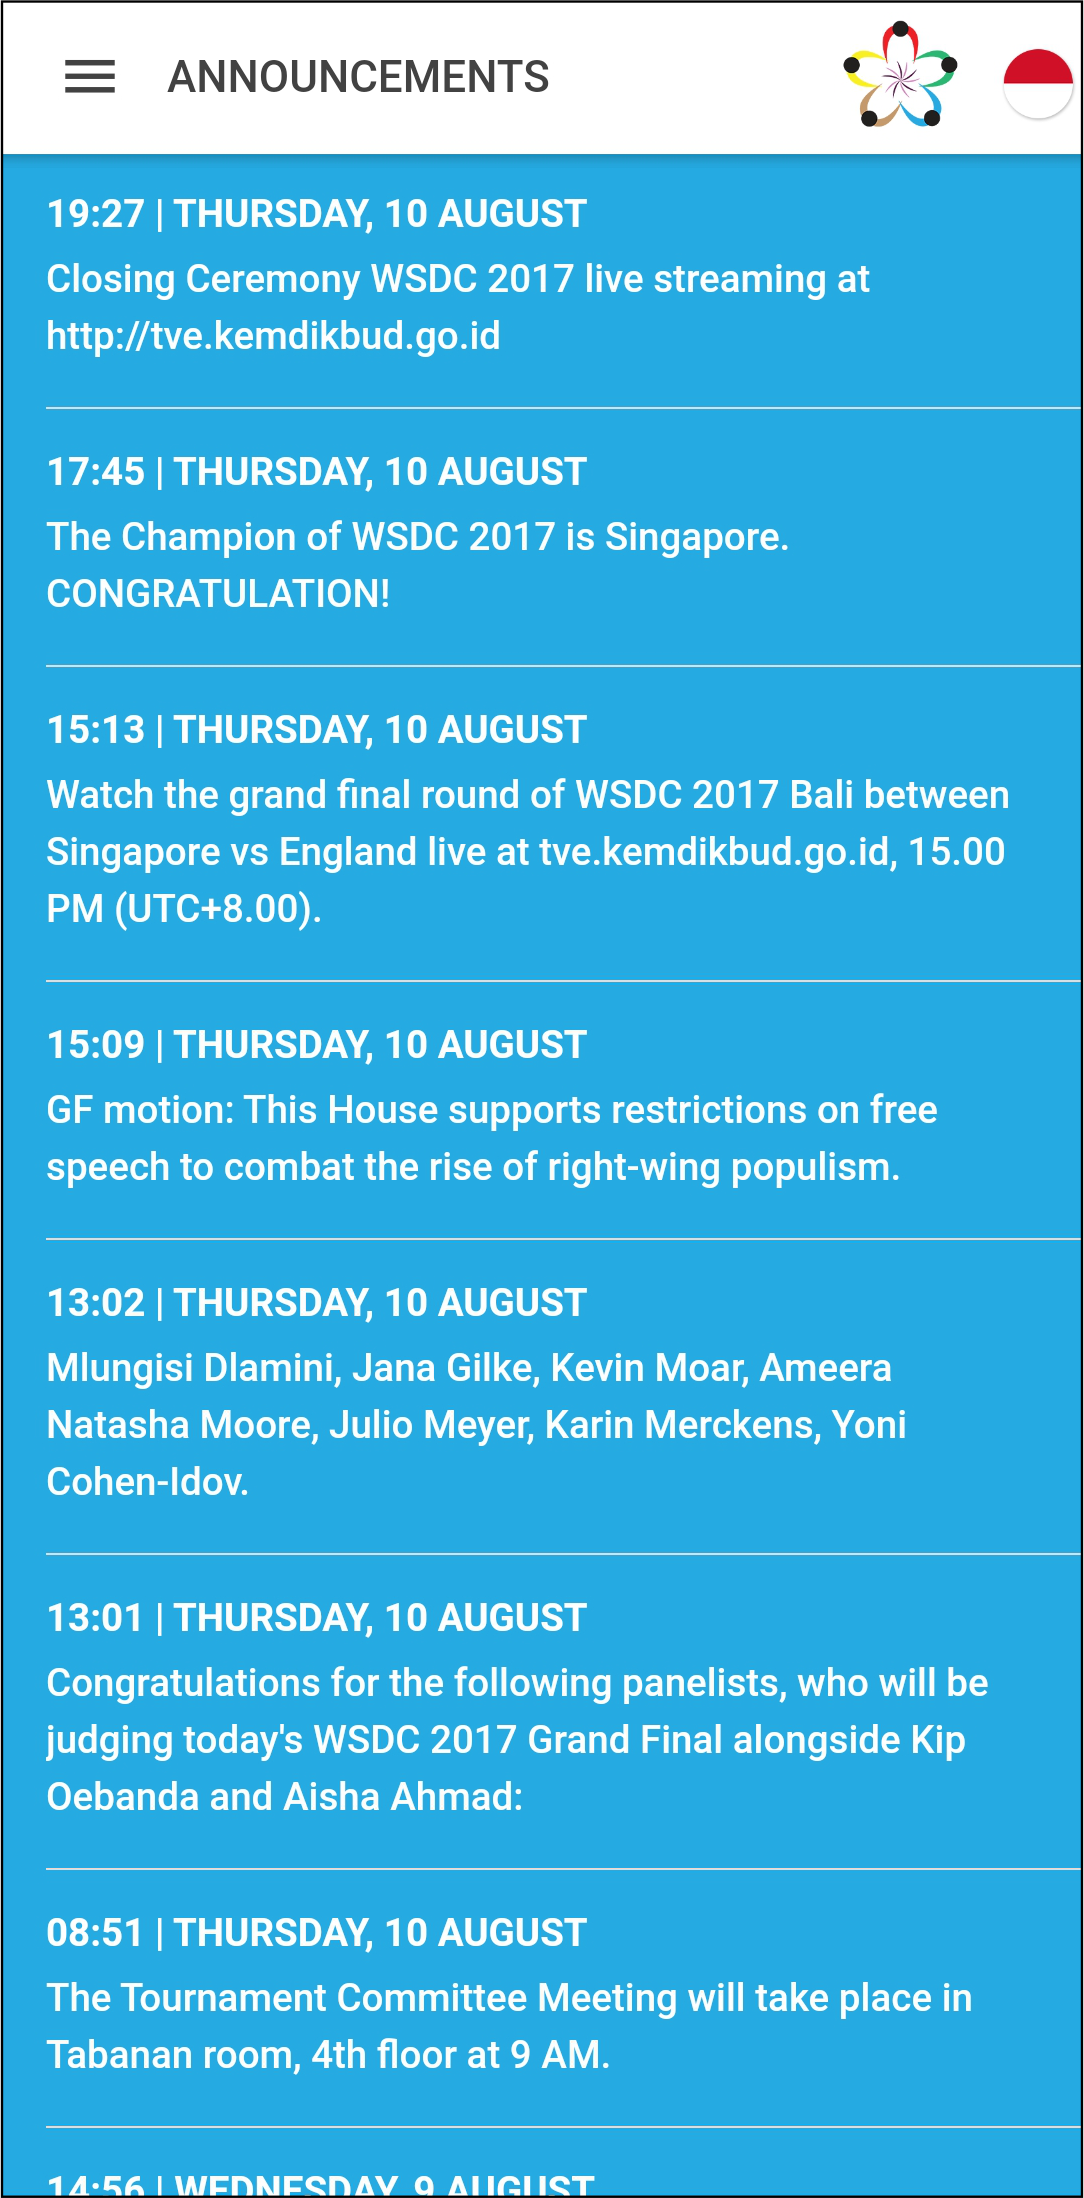
\includegraphics[scale=0.37]{Gambar/AnnouncementsPage.png}
	    \caption{\textit{Announcements Page}}
	    \label{fig:wsdcAppAnnouncements}
     \end{subfigure}
	\begin{subfigure}[b]{0.24\textwidth}
    \centering
	    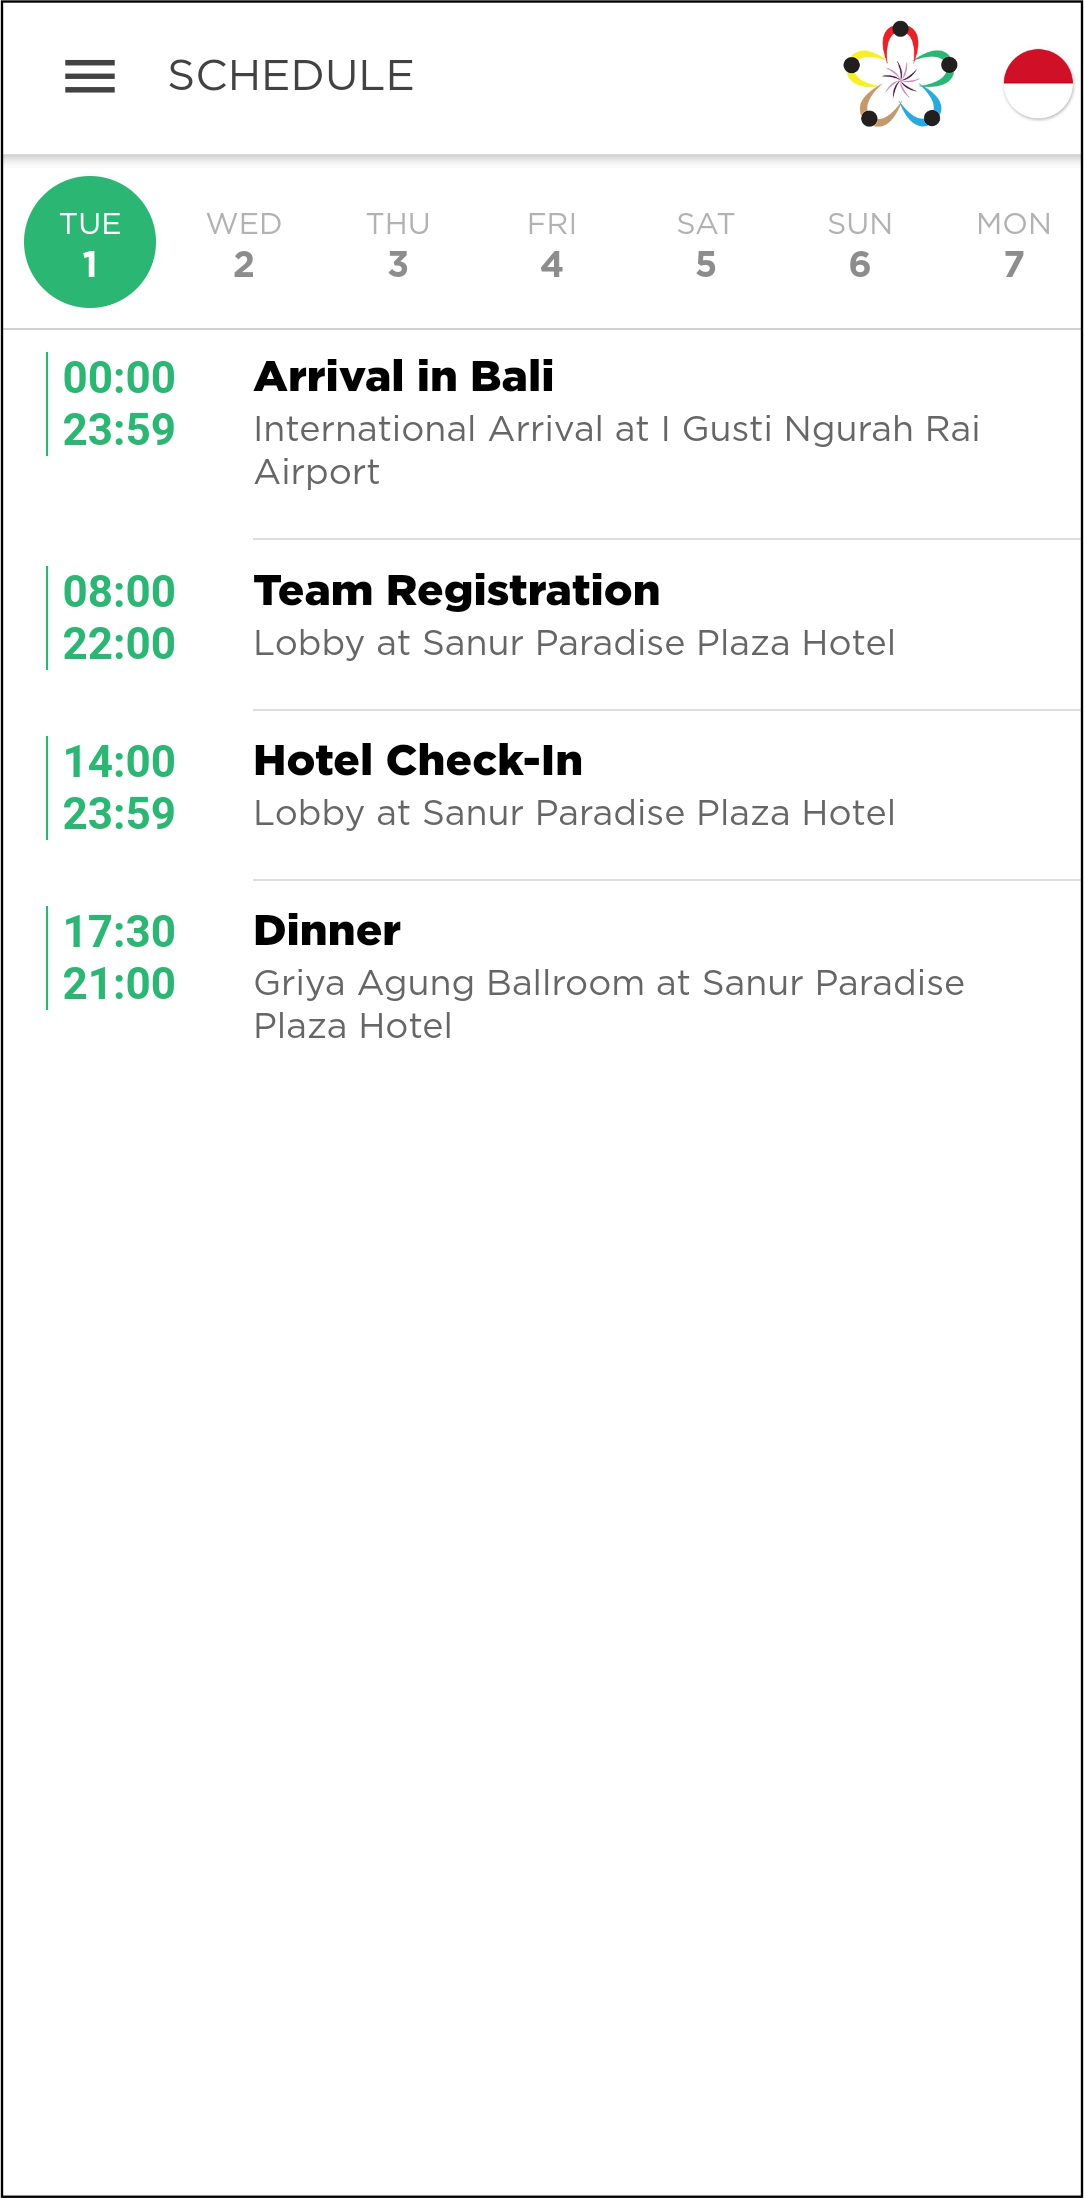
\includegraphics[scale=0.37]{Gambar/SchedulePage.png}
	    \caption{{\it Schedule Page}}
	    \label{fig:wsdcAppSchedule}
     \end{subfigure}
	\begin{subfigure}[b]{0.24\textwidth}
    \centering
	    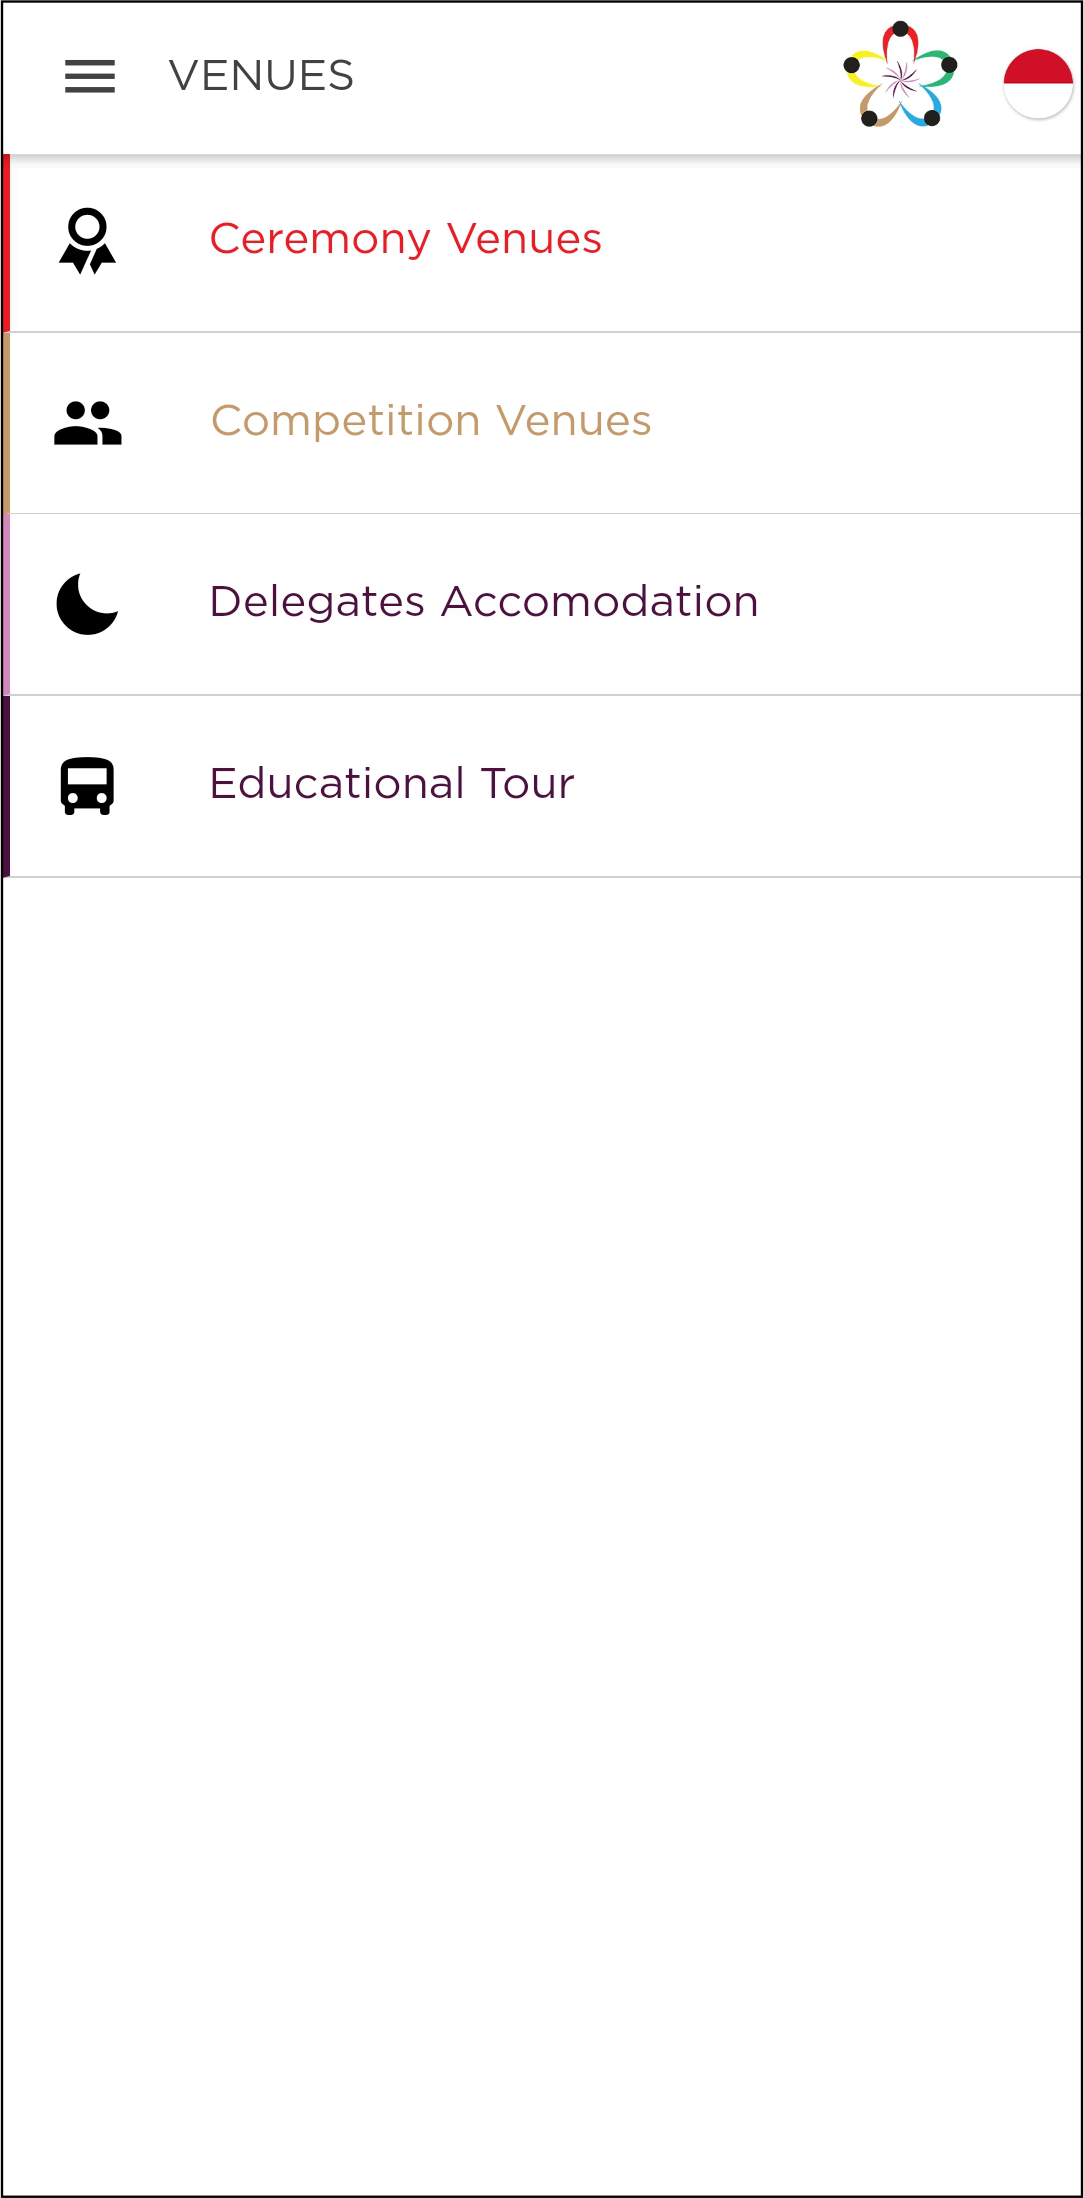
\includegraphics[scale=0.37]{Gambar/VenuePage.png}
	    \caption{\textit{Venues Page}}
	    \label{fig:wsdcAppVenues} 
     \end{subfigure}
	\caption{Aplikasi WSDC 2017 Bali Saat Ini pada Perangkat Android}
        \label{fig:ssAppWSDC2017Bali2}
\end{figure}

Fitur-fitur yang terdapat di aplikasi WSDC 2017 Bali saat ini yaitu :

\begin{enumerate}
	\item \textit{Home Page}: Pengguna dapat melihat pengumuman terbaru, dan \textit{headline} dari berita-berita terkait acara WSDC 2017 Bali dengan tombol yang dapat diklik untuk melihat berita tersebut secara lebih detail (Gambar~\ref{fig:wsdcapp}).

	\item {\it Announcements}: Pengguna dapat melihat pemberitahuan tentang berjalannya acara WSDC 2017 Bali (Gambar~\ref{fig:wsdcAppAnnouncements}).

	\item {\it Schedule}: Pengguna dapat melihat jadwal acara WSDC 2017 Bali yang sudah diadakan (Gambar~\ref{fig:wsdcAppSchedule}).

	\item {\it Venues}: Pengguna dapat melihat berbagai macam lokasi acara WSDC 2017 Bali, mulai dari lokasi upacara, lokasi kompetisi, dan lokasi wisata edukasi (Gambar~\ref{fig:wsdcAppVenues}). Masing-masing dari lokasi tersebut ditunjukkan dengan tanda merah pada peta dan dapat melihat jarak dari lokasi perangkat pengguna ke lokasi \textit{venues} (Gambar~\ref{fig:wsdcAppVenuesMap}).

	\item Info: Pengguna dapat melihat informasi terkait dengan tim pengembang dari aplikasi WSDC 2017 Bali, kontak-kontak penting yang dapat dihubungi, dan kosa kata penting dalam Bahasa Indonesia (Gambar~\ref{fig:wsdcAppInfo}).

	\item {\it Draw}: Pengguna dapat melihat melihat pembagian {\it venue} dan kubu proposisi atau oposisi dari hasil pengundian untuk para negara peserta WSDC 2017 Bali (Gambar~\ref{fig:wsdcAppDraw}).

	\item {\it Result}: Pengguna dapat melihat informasi terkait hasil dari pertandingan pada semi final, perempat final, dan perdelapan final WSDC 2017 Bali (Gambar~\ref{fig:wsdcAppResult}).
\end{enumerate}

\begin{figure}[H]
     \centering
     \begin{subfigure}[b]{0.21\textwidth}
        \centering
	    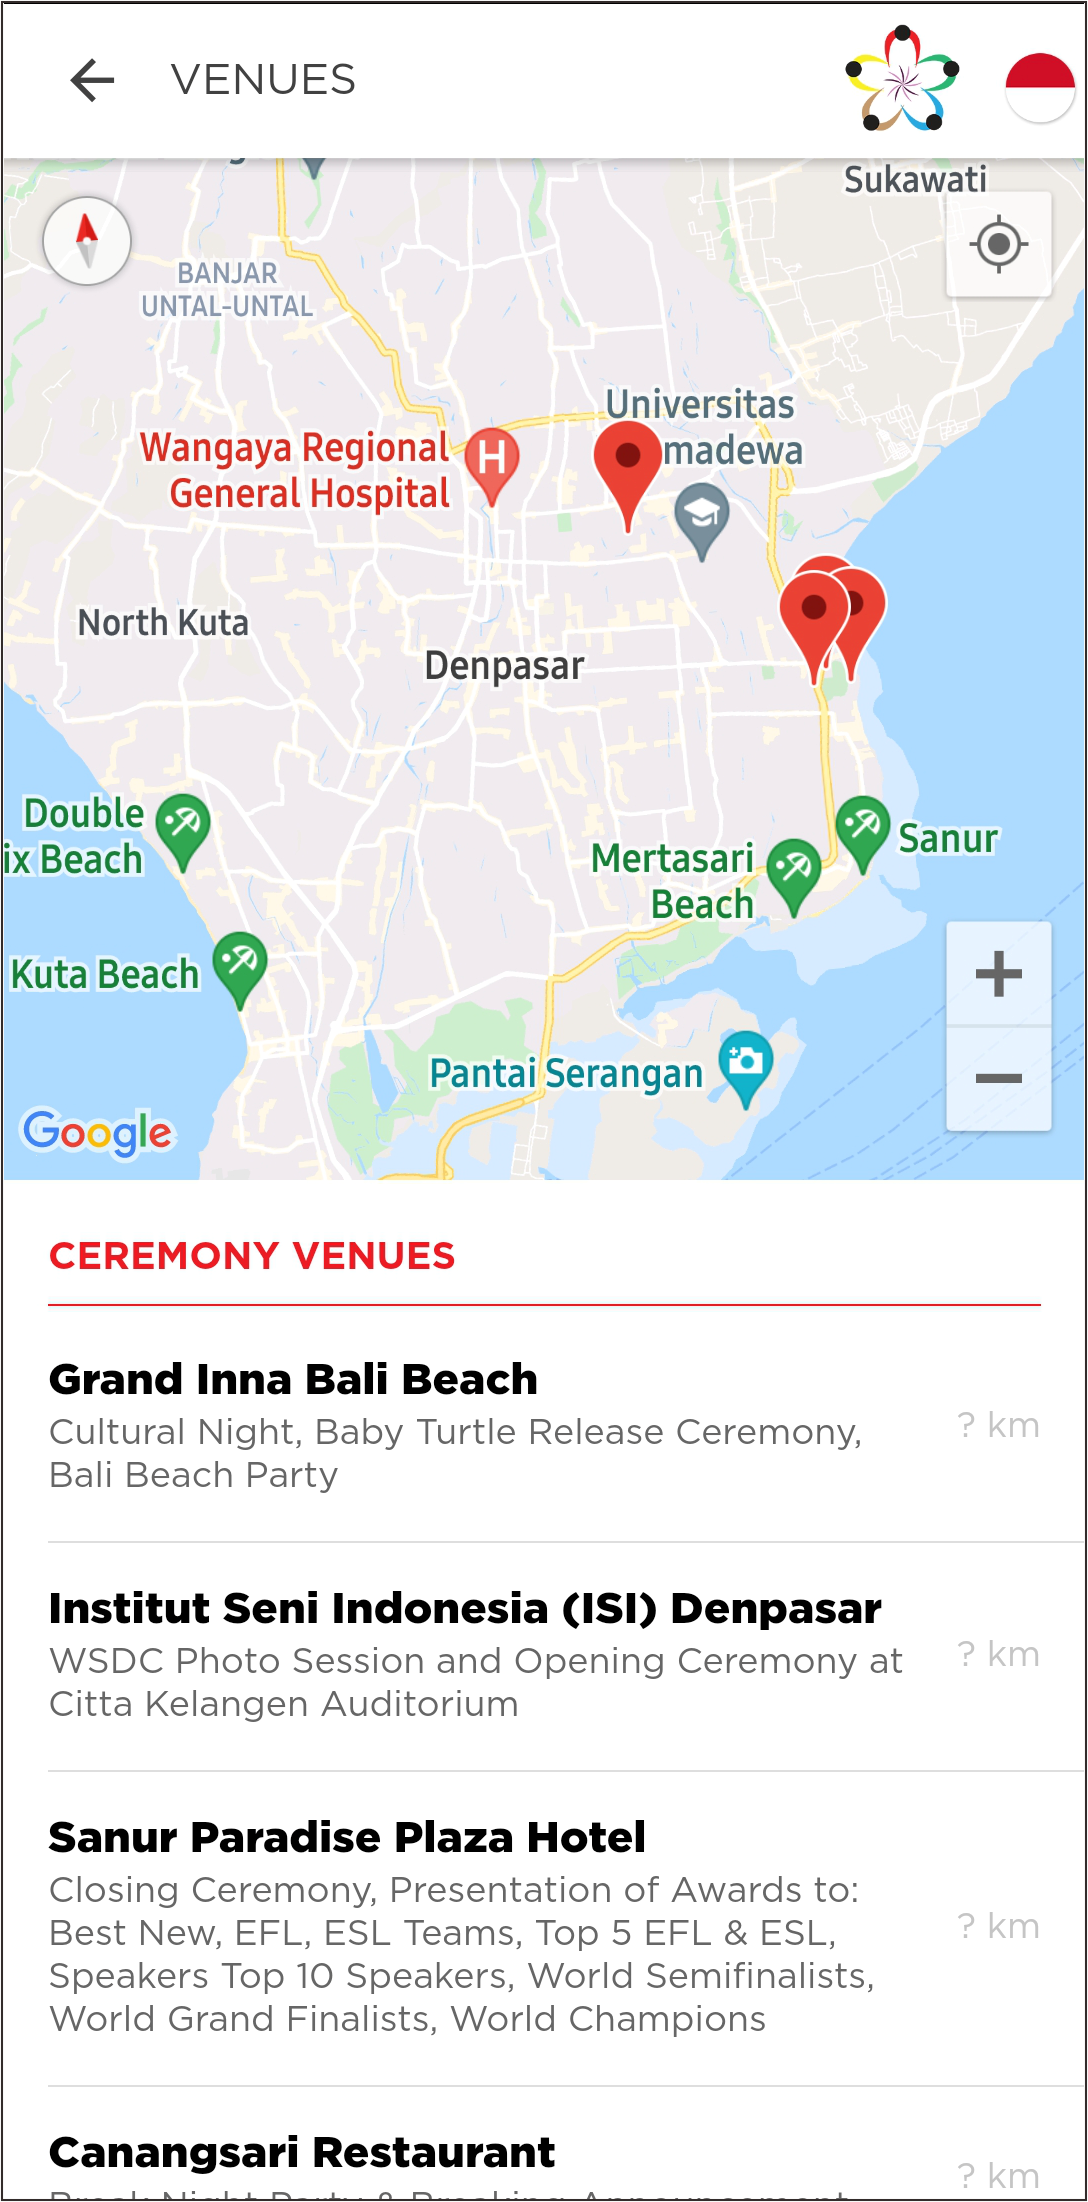
\includegraphics[scale=0.4]{Gambar/VenuesMapPage.png}
	    \caption{{\it Venues Map Page}}
	    \label{fig:wsdcAppVenuesMap}
     \end{subfigure}
     \hfill
     \begin{subfigure}[b]{0.247\textwidth}
    \centering
	    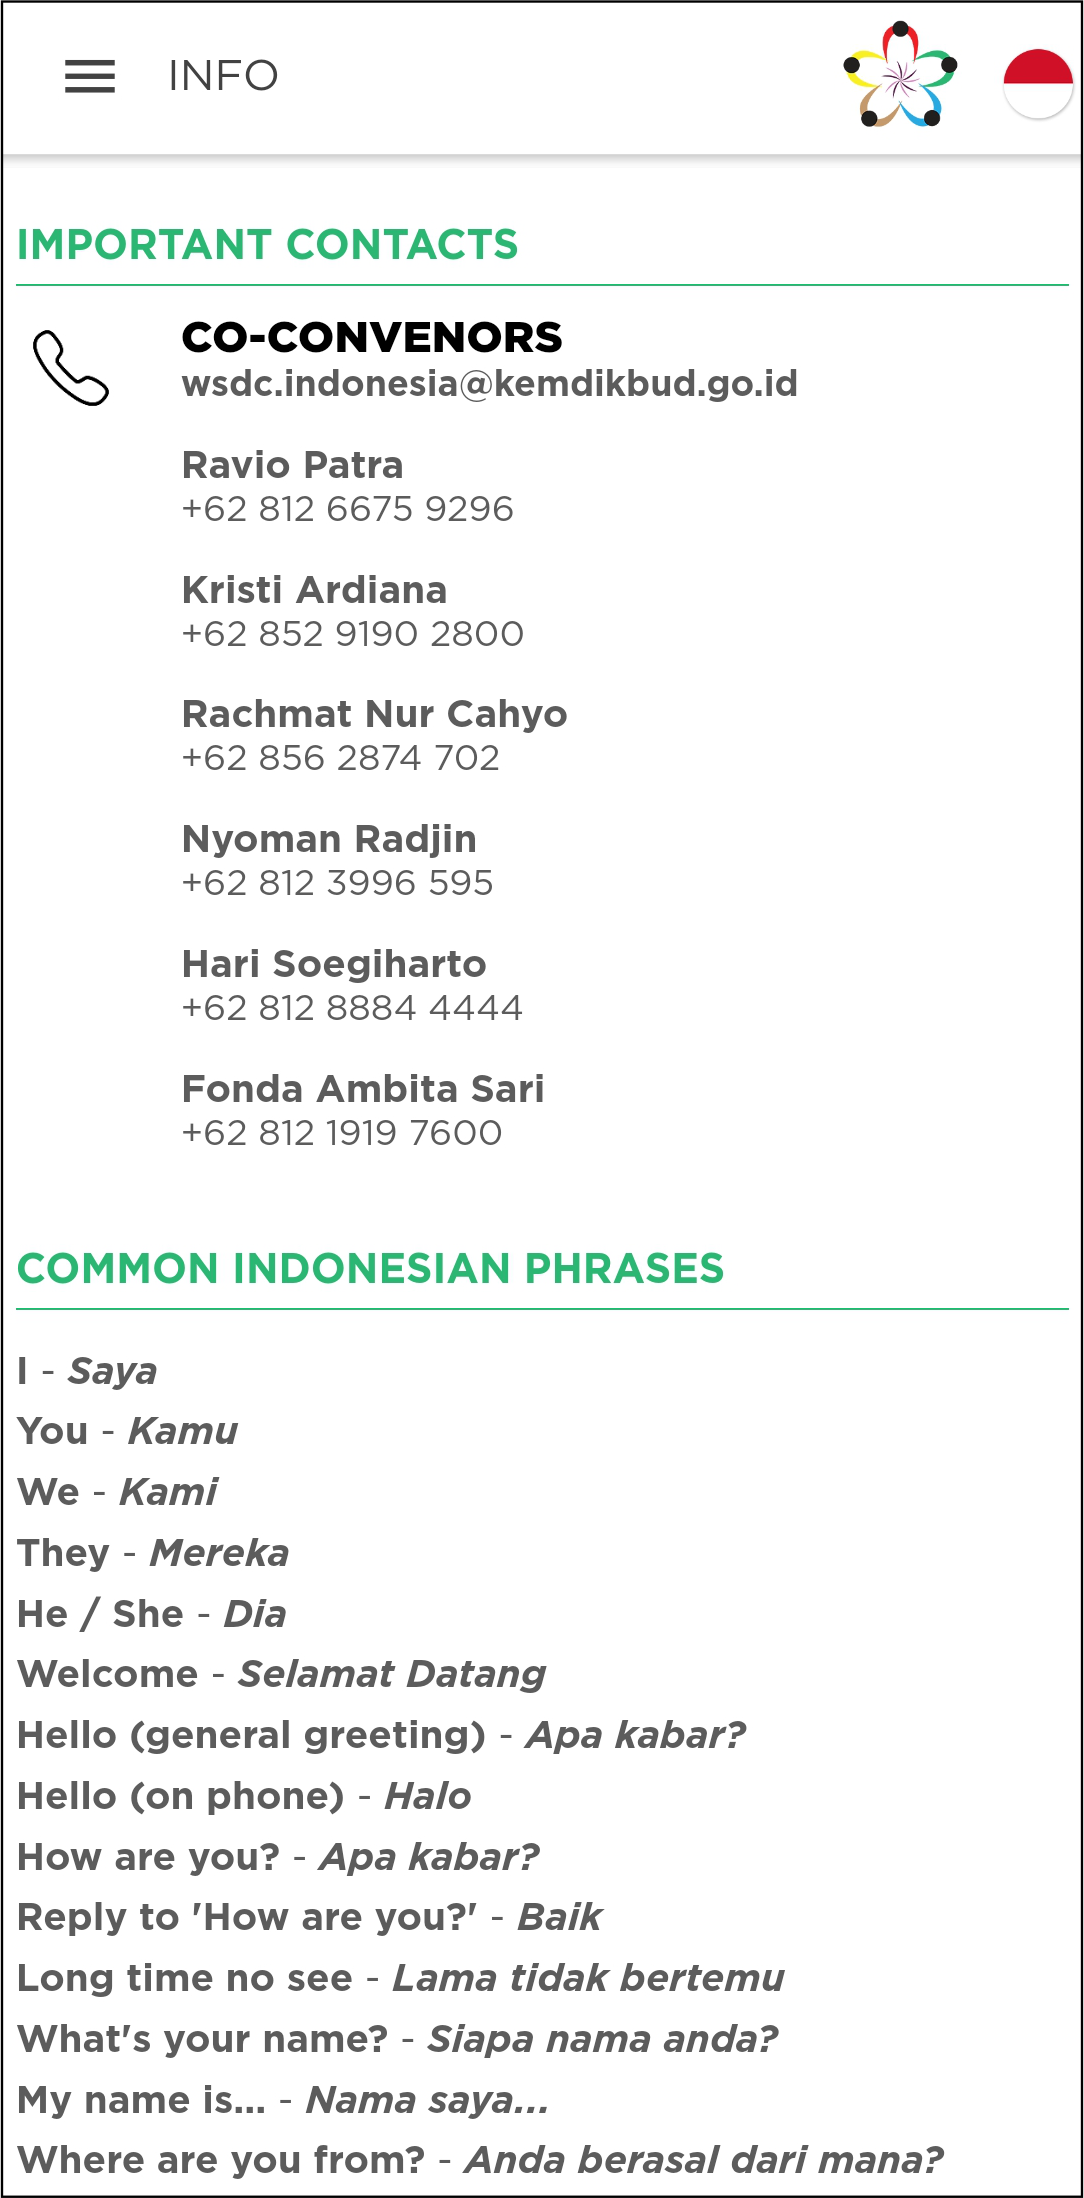
\includegraphics[scale=0.4]{Gambar/InfoPage.png}
	    \caption{Info \textit{Page}}
	    \label{fig:wsdcAppInfo}
     \end{subfigure}
	\begin{subfigure}[b]{0.247\textwidth}
    \centering
	    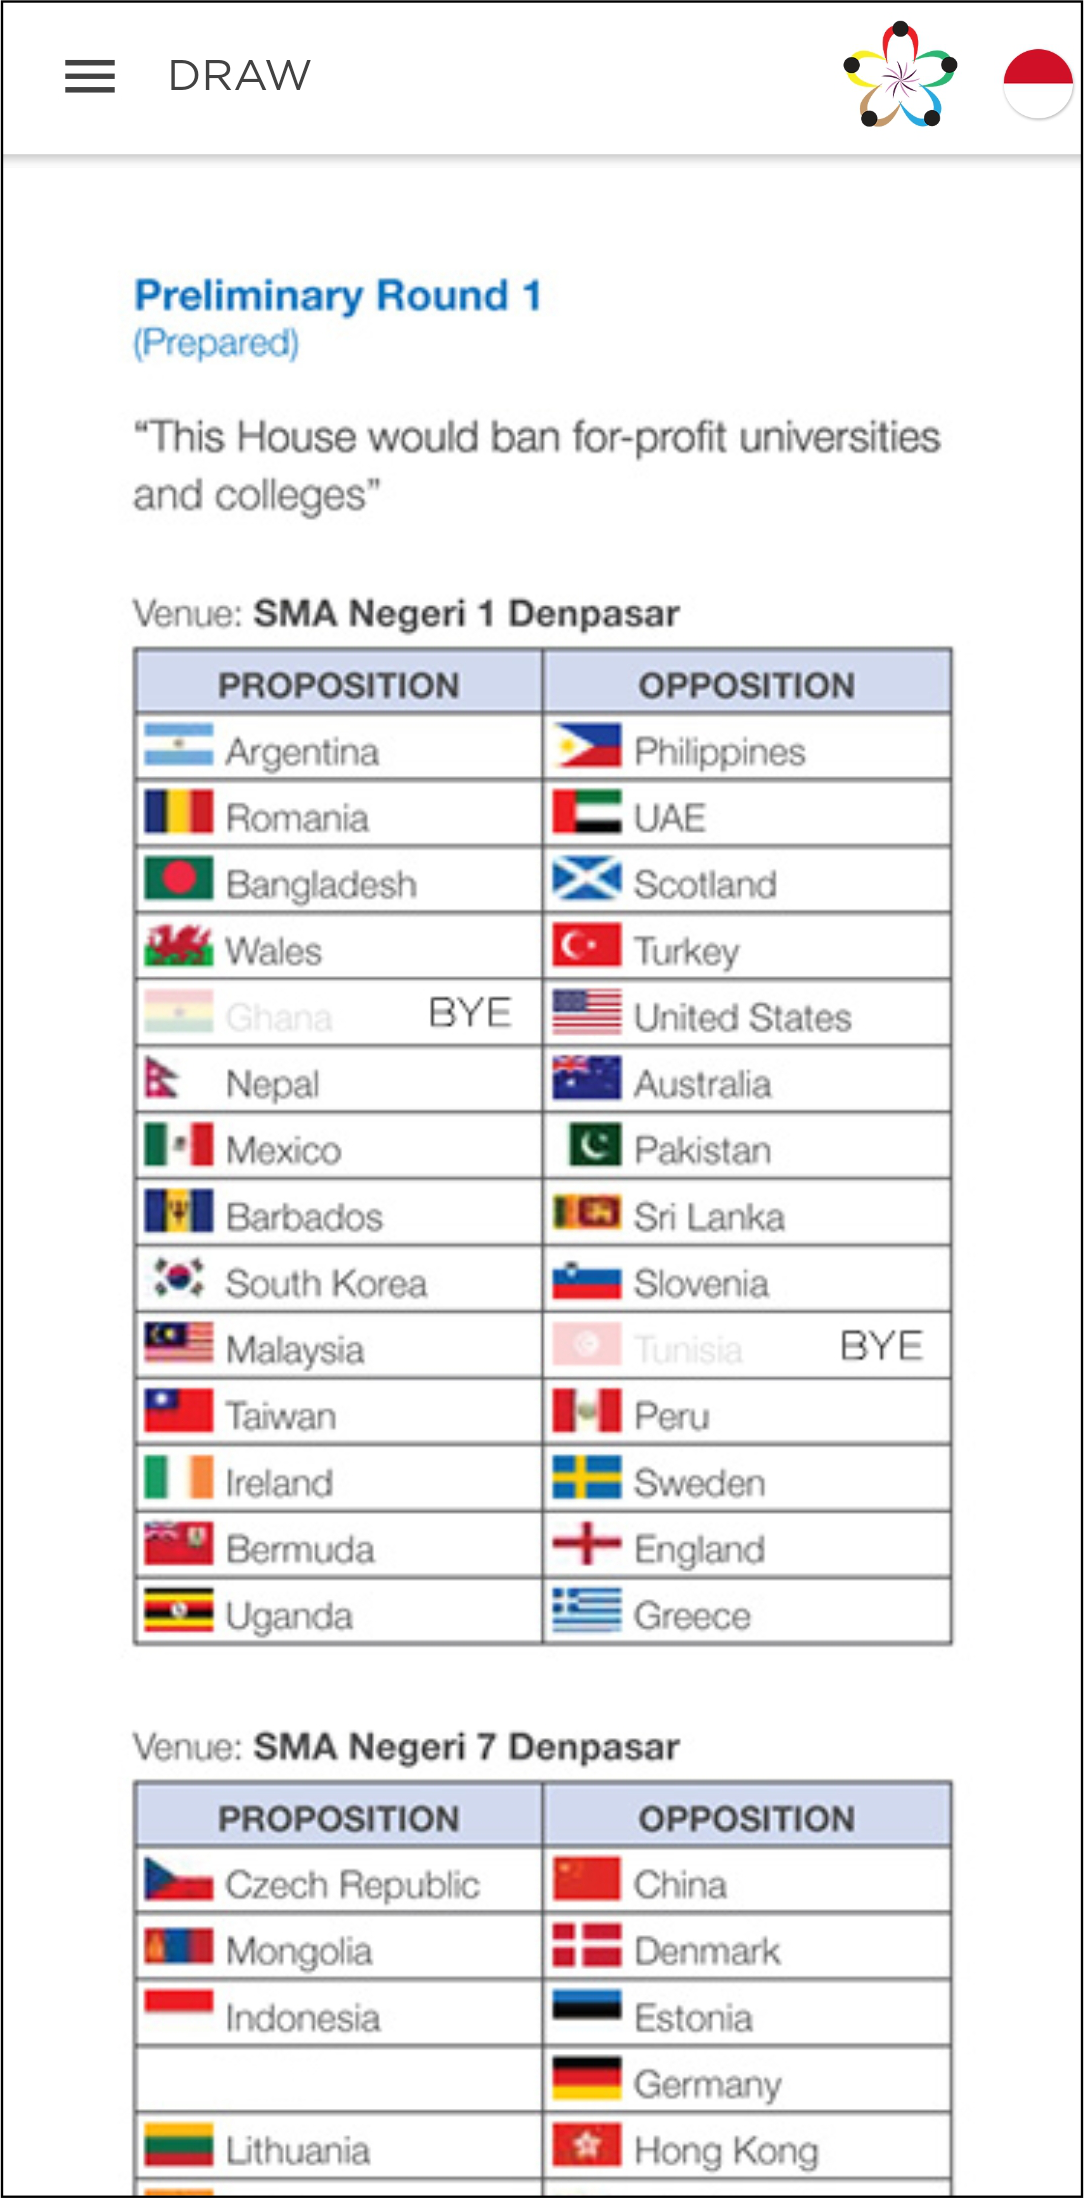
\includegraphics[scale=0.4]{Gambar/DrawPage.png}
	    \caption{{\it Draw Page}}
	    \label{fig:wsdcAppDraw}
     \end{subfigure}
	\begin{subfigure}[b]{0.247\textwidth}
    \centering
	    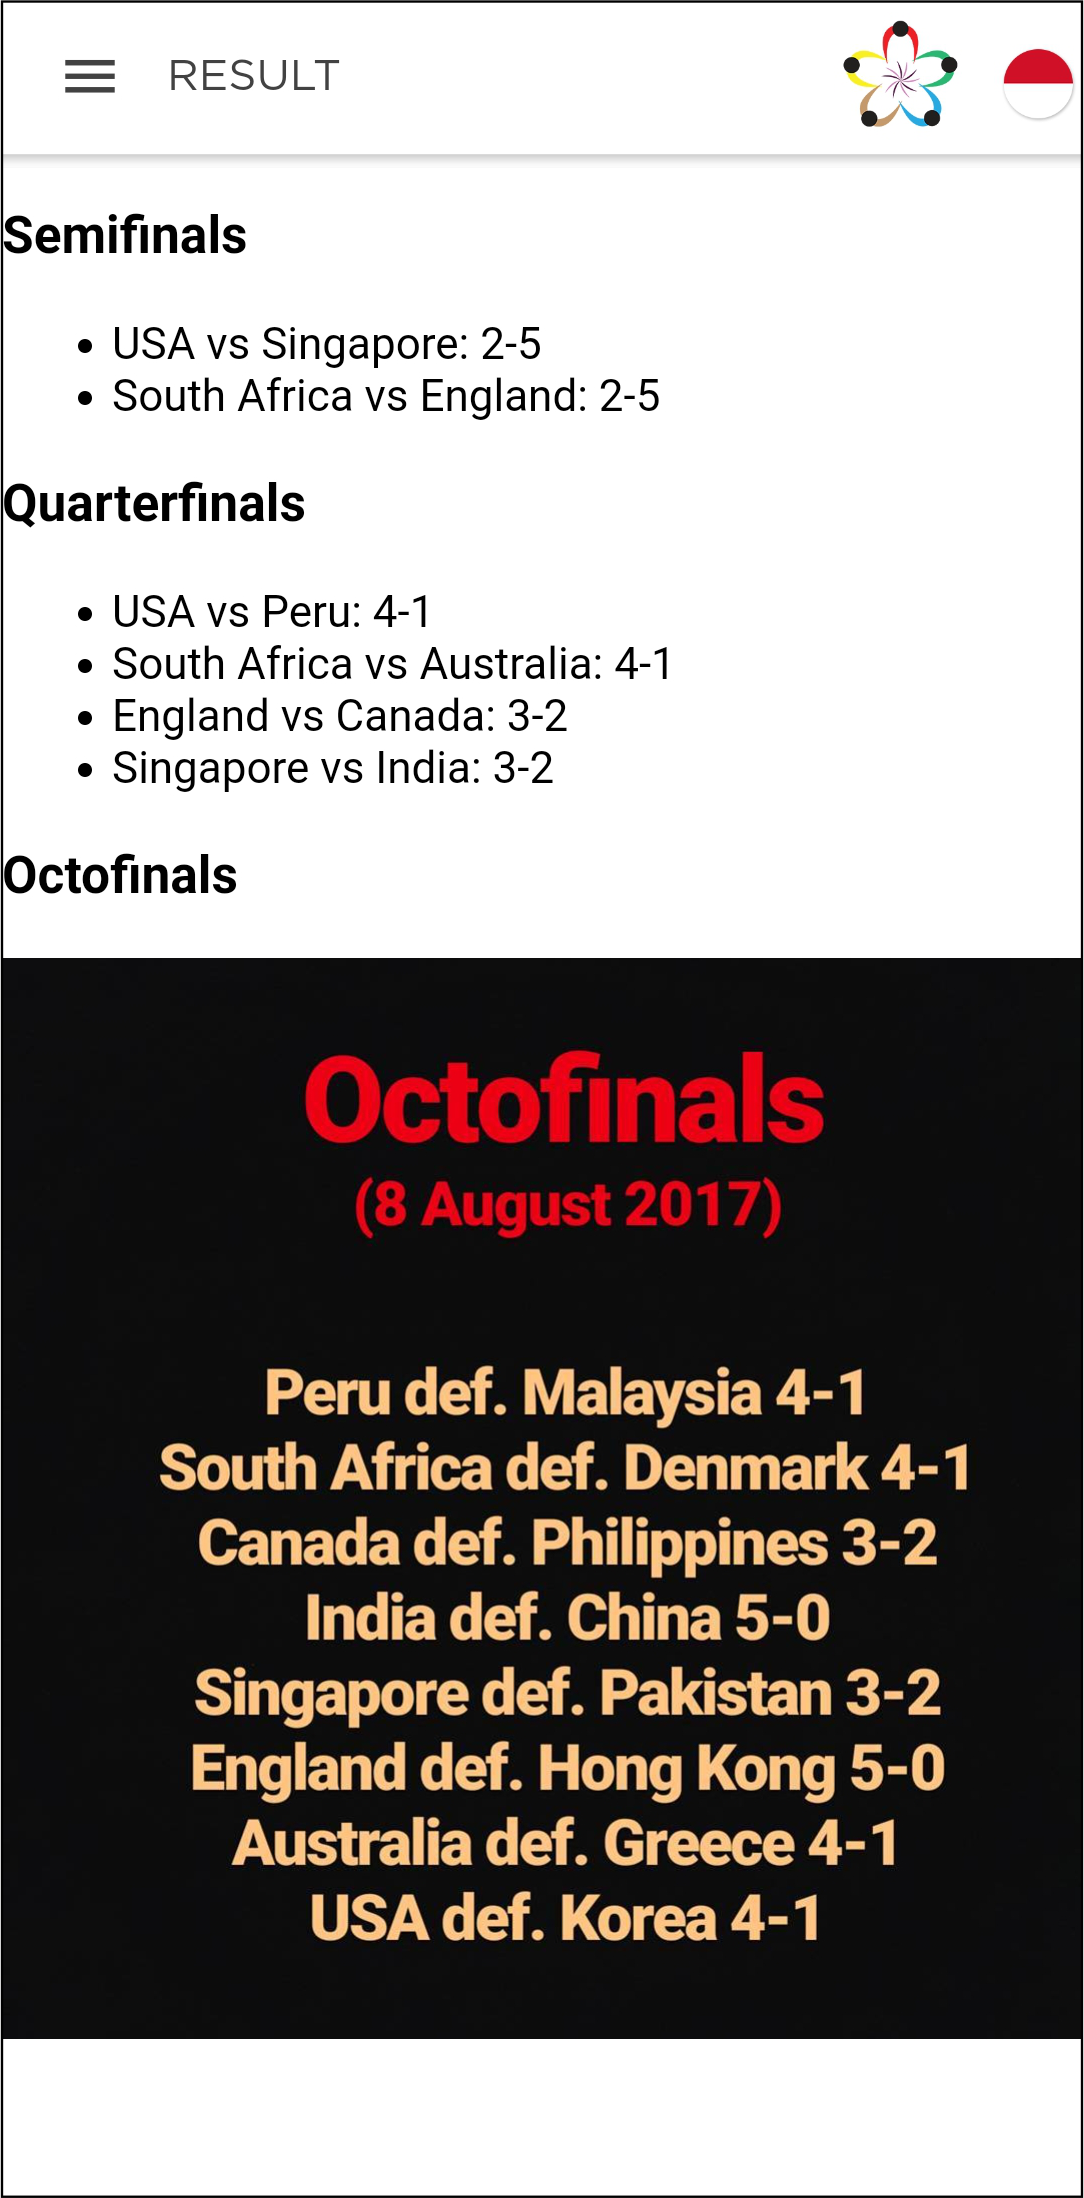
\includegraphics[scale=0.4]{Gambar/ResultPage.png}
	    \caption{{\it Result Page}}
	    \label{fig:wsdcAppResult}
     \end{subfigure}
	\caption{Aplikasi WSDC 2017 Bali Saat Ini pada Perangkat Android}
        \label{fig:ssAppWSDC2017Bali2}
\end{figure}

\section{Angular}
\label{sec:angular} 
%buku Angular Development with TypeScript
Angular merupakan \textit{framework} Javascript terbuka yang dikembangkan oleh Google, dan merupakan penerus dari versi sebelumnya yaitu AngularJS~\cite{fain:18:angular}. Angular versi pertama dirilis pada tahun 2016 dengan nama Angular 2. Aplikasi Angular dapat dibangun dengan menggunakan JavaScript, atau TypeScript.

\begin{figure}[H]
		\centering
	    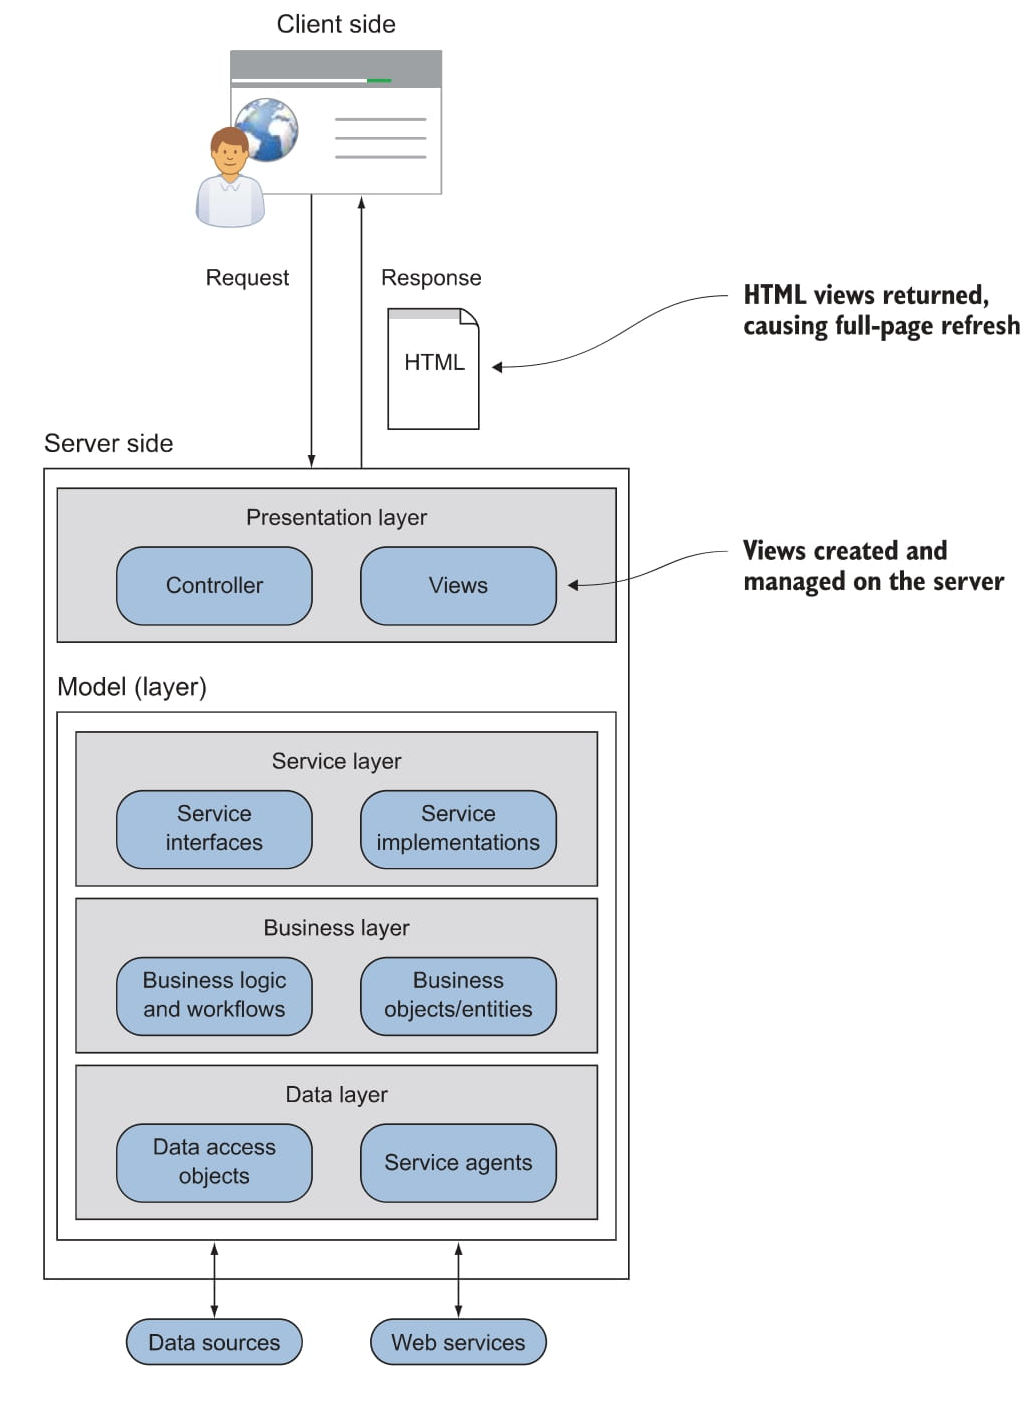
\includegraphics[scale=0.9]{Gambar/tradisionaldesain.png}
	    \caption{Desain \textit{server-side} tradisional~\cite{scott:15:spa}}
	    \label{fig:tradisionaldesain}
\end{figure}

%buku SPA Design and Architecture: Understanding single-page web applications
Angular dapat digunakan untuk membuat aplikasi Single-page-application (SPA), yaitu ketika halaman awal dimuat, semua yang dibutuhkan untuk membuat dan menampilkan sebuah halaman diunduh, kemudian ditampilkan kedalam layar~\cite{scott:15:spa}. Website dengan desain SPA berbeda dengan desain tradisional. Seperti pada Gambar~\ref{fig:tradisionaldesain}, pada desain tradisional setiap permintaan untuk tampilan baru, yaitu halaman HTML, memerlukan \textit{request} ke server dan mengembalikannya kembali ke \textit{client}. Ketika data baru diperlukan oleh \textit{client}, permintaan dikirim ke sisi server. Di sisi server, permintaan diambil oleh \textit{controller} di dalam \textit{presentation layer}.

\textit{Controller} kemudian berinteraksi dengan \textit{model layer} melalui \textit{service layer} untuk menentukan data yang diperlukan. Permintaan terhadap data tersebut diteruskan ke \textit{data layer} yang kemudian mengambil data dari \textit{web service}. Setelah data diambil, setiap perubahan yang diperlukan pada data kemudian dibuat oleh \textit{business logic} di \textit{business layer}. Lalu setelah perubahan yang diperlukan pada data telah selesai di \textit{business logic}, data dikembalikan ke \textit{presentation layer}. Di dalam \textit{presentation layer} menentukan bagaimana data yang baru diperoleh direpresentasikan ke dalam tampilan yang dipilih. Setelah data dan tampilan digabungkan, tampilan dikembalikan ke browser. Browser kemudian menerima halaman HTML setelah melakukan \textit{refresh} pada tampilan antarmuka \textit{browser}. Pada akhirnya pengguna melihat tampilan baru yang berisi data yang diminta setelah \textit{browser} melakukan \textit{refresh}.

\begin{figure}[H]
		\centering
	    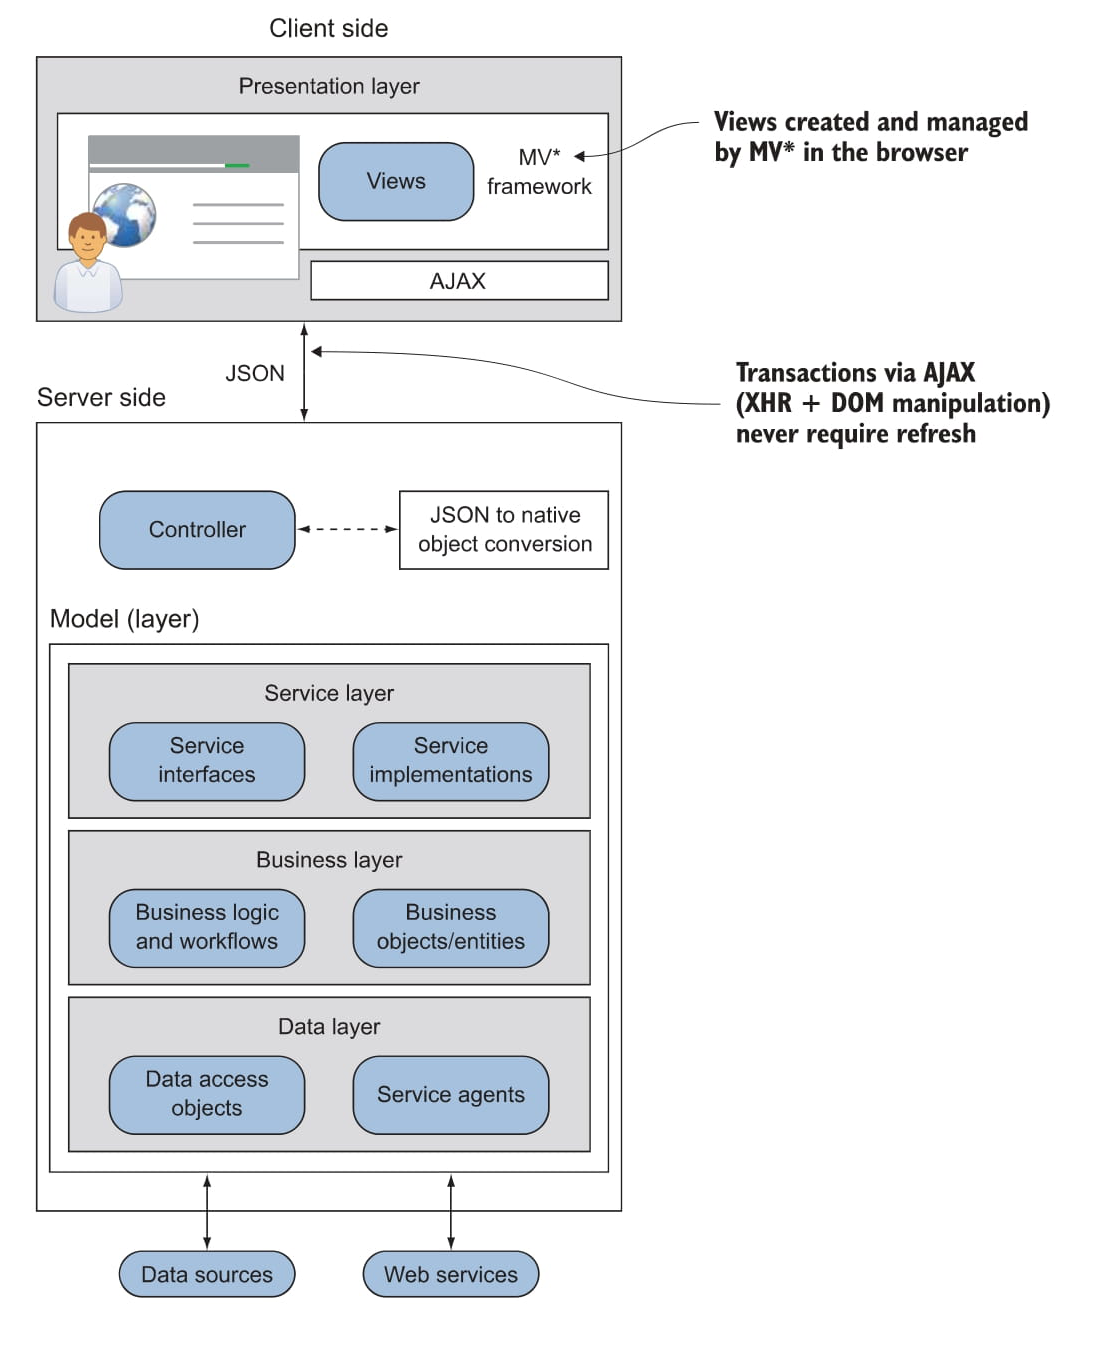
\includegraphics[scale=0.9]{Gambar/spadesain.png}
	    \caption{Desain SPA~\cite{scott:15:spa}}
	    \label{fig:spadesain}
\end{figure}

Pada desain SPA, pengelolaan tampilan antarmuka dan server terpisah seperti pada Gambar~\ref{fig:spadesain}. Hal tersebut membuat desain SPA hampir sama dengan desain tradisional, namun terdapat perbedaan berupa tidak ada lagi \textit{refresh} pada \textit{browser} untuk mendapatkan tampilan halaman dengan data yang baru, dan \textit{presentation layer} berada di \textit{client} yang membuat tugas menggabungkan HTML dan data dipindahkan dari server ke browser. Pada desain SPA, setelah halaman awal dimuat, semua data yang diperlukan untuk membuat dan menampilkan tampilan diunduh dan siap digunakan. Jika diperlukan tampilan baru, tampilan tersebut dibuat secara lokal di browser dan ditampilkan secara dinamis melalui JavaScript sehingga tidak diperlukan \textit{refresh} pada browser.

%Nulis typiscrript
Angular dapat dibangun dengan menggunakan JavaScript atau TypeScript. Namun, penggunaan TypeScript saat ini menjadi lebih produktif dibandingkan dengan JavaScript~\cite{fain:18:angular}. TypeScript mengikuti perkembangan terakhir dari ECMAScript, yaitu bahasa skrip yang distandarisasi oleh Ecma International dalam spesifikasi ECMA-262 dan ISO/IEC 16262~\cite{rarayan:15:learning}. TypeScript juga menambahkan \textit{types}, \textit{interface}, \textit{decorators}, \textit{class member variables}, \textit{generic}, \textit{enum}, dan \textit{keyword} seperti \textit{public}, \textit{protected}, dan \textit{private} serta dapat digunakan untuk mendeklarisasi jenis tipe khusus yang dapat di kustomisasi. Maka dari itu, Framework Angular sendiri ditulis menggunakan TypeScript.

Angular terdiri dari komponen-komponen yang merupakan sebuah penyusun utama untuk aplikasi Angular. Setiap komponen yang ada pada aplikasi, secara \textit{default} memiliki \textit{critical files} yang terdiri dari \textit{file} HTML untuk mendeklarasi halaman yang akan dimuat, \textit{file} TypeScript, serta \textit{file} css~\cite{gion:18:mastering}. Di dalam komponen terdapat module.ts yang merupakan NgModule dari sebuah komponen, spec.ts yang digunakan untuk menguji komponen, dan routing.module.ts yang berisi definisi untuk bernavigasi antar bagian dalam aplikasi Angular. Penjelasan untuk masing-masing \textit{file} adalah sebagai berikut:

\begin{itemize}
	\item \textit{File} routing.module.ts \\
		\textit{File} ini digunakan untuk melakukan navigasi antar komponen. Untuk melakukannya, harus melakukan \textit{import} RouterModule dan Routes sehingga dapat memiliki fungsionalitas \textit{routing}~(Kode~\ref{lst:importroutingmodule}). Pada kode tersebut, dilakukan \textit{import} RouterModule dan Routes dari @angular/router. Selanjutnya lakukan \textit{import} untuk komponen lain yang akan dituju untuk melakukan navigasi ke komponen tersebut. Sebagai contoh, pada kode~\ref{lst:importroutingmodule} melakukan \textit{import} untuk komponen ``Heroes``.

\begin{lstlisting}[label={lst:importroutingmodule}, caption={Contoh \textit{import} pada routing.module.ts}]
import { RouterModule, Routes } from '@angular/router';
import { HeroesComponent } from './heroes/heroes.component';
\end{lstlisting} 

		Setelah itu, lakukan konfigurasi \textit{routes}. Routes kemudian memberi tahu Router tampilan mana yang akan ditampilkan saat pengguna melakukan navigasi. Seperti pada kode~\ref{lst:confroutingmodule}, dengan menggunakan key path dan component. Path digunakan untuk melakukan navigasi di alamat url sesuai dengan path tersebut. Sedangkan component digunakan untuk menampilkan komponen yang dituju.
		
\begin{lstlisting}[label={lst:confroutingmodule}, caption=Contoh Konfigurasi \textit{Routes} pada routing.module.ts, captionpos=b]
const routes: Routes = [
  { path: 'heroes', component: HeroesComponent }
];
\end{lstlisting} 

	\item \textit{File} CSS \\
		\textit{File} ini digunakan sebagai \textit{template} CSS untuk sebuah komponen. Aplikasi angular ditata dengan CSS standar, yang dapat menerapkan  semua CSS stylesheets, \textit{selectors}, \textit{rules}, dan \textit{media queries} langsung ke aplikasi Angular.
		 
	\item \textit{File} HTML \\
		\textit{File} HTML pada Angular sama seperti HTML biasa, dan bisa ditambahkan dengan sintaks Angular. HTML pada komponen digunakan untuk mendeklarasi halaman yang akan dimuat.
		
	\item \textit{File} specs.ts \\
		\textit{File} ini digunakan untuk melakukan pengujian terhadap aplikasi Angular. 
		
	\item \textit{File} TypeScript \\
		Di dalam TypeScript, terdapat sebuah kelas komponen. Kelas tersebut memiliki anotasi dengan sebuah \textit{decorator}~(Kode~\ref{lst:decorator}) yang ditempatkan sesuai dengan komponen UI nya berada. Komponen berisi \textit{instance} dari service class yang diimplementasi dari \textit{business logic} tanpa UI. Sebuah service class merupakan implementasi dari \textit{business logic}. Angular akan menempatkan \textit{services} ke dalam komponen atau ke dalam \textit{services} lainnya dengan menggunakan \textit{dependency injection} (DI). 	

\begin{lstlisting}[label={lst:decorator}, caption=Anotasi Komponen dengan \textit{Decorator}]
@Component({
	...
}
export class AppComponent{
	...
})
\end{lstlisting} 

		Pada Angular terdapat decorator @Component yang digunakan untuk memanggil HTML \textit{template} dan CSS untuk komponen. Pada setiap komponen terdapat HTML \textit{template} yang berada di dalam komponen tersebut, atau di dalam file yang berada di luar file kopmonen yang direferensikan dengan menggunakan properti \textbf{templateUrl} di dalam komponen pada \textit{file} TypeScript. File HTML \textit{template} yang terpisah dengan komponen, memberikan efek kode yang lebih bersih di dalam komponen nya. Selain HTML \textit{template}, file lain seperti file CSS dapat diletakan terpisah dari file komponen dengan menggunakan styleUrls untuk mereferensikan file CSS ke dalam komponen (Kode~\ref{lst:referensiHTMLCSSdiKomponen}). Lalu terdapat juga properti selector untuk mendefinisikan nama dari tag yang bisa digunakan atau dipanggil oleh komponen lain.

\begin{lstlisting}[label={lst:referensiHTMLCSSdiKomponen}, caption=Contoh Mereferensikan HTML dan CSS di Dalam Komponen]
@Component({
	selector: 'app-search',
	templateUrl: './search.component.html',
	styleUrl:['./search.component.css']
})
export class SearchComponent{
	...
}
\end{lstlisting} 

	\item \textit{File} module.ts \\
	Komponen-komponen yang ada akan dikelompokkan menjadi Angular modules, yaitu sebuah kelas yang diberi \textbf{@NgModule()}. Angular module biasanya merupakan sebuah kelas kecil yang tidak memiliki isi, kecuali menulis kode bootstrap secara manual ke dalam aplikasi. Contohnya, ketika sebuah aplikasi merupakan turunan dari AngularJS yang lama, \textit{decorator} \textbf{@NgModule()} menampilkan semua komonen dan \textit{artifacts} lain termasuk \textit{services}, \textit{directive}, dan yang lainnya, maka semua itu harus disertakan ke dalam module (Kode~\ref{lst:moduleComponent}). 

\begin{lstlisting}[label={lst:moduleComponent}, caption=Module dengan Komponen]
@NgModule({
	declaration: [
		AppComponent
	],
	imports: [
		BrowserModule	
	],
	bootstrap: [AppComponent]
})
export class AppModule{
	...
}
\end{lstlisting} 
\end{itemize}

Di dalam aplikasi Angular, terdapat beberapa komponen, seperti Parent Component, dan Child Component. Parent Component dapat mengirimkan data ke properti Child Component-nya. Namun, Child Component tidak tahu siapa yang mengirimkannya. Sedangkan Child Component juga dapat mengirimkan data ke Parent Component, meskipun dia tidak tahu siapa Parent Component-nya. Arsitektur seperti ini dapat membuat komponen menjadi mandiri dan dapat digunakan kembali.

\newpage

Angular menyediakan beberapa \textit{libraries}, yaitu:

\begin{enumerate}
	\item Angular Router \\
	Angular Router digunakan untuk menangani navigasi dari satu tampilan ke tampilan lain, dan kemudian menampilkannya di layar~\cite{victor:17:angular}. Langkah-langkah untuk membuat \textit{route} pada Angular adalah sebagai berikut:
	
	\begin{enumerate}
		\item Import RouterModule dan Routes ke routing module. \\
		Pada tahap ini, Angular CLI membuatnya secara otomatis saat pembuatan proyek Angular. Angular CLI membuat array Routes, dan melakukan import serta export array di @NgModule(). Seperti pada contoh kode~\ref{lst:angularRouting} pada baris ke-2 dilakukan import untuk Routes dan RouterModule dari Angular, serta pada baris ke-4 Angular CLI membuat array Routes.
		
\begin{lstlisting}[label={lst:angularRouting}, caption={Contoh \textit{Routing} pada Angular}]
import { NgModule } from '@angular/core';
import { Routes, RouterModule } from '@angular/router';

const routes: Routes = []; 

@NgModule({
  imports: [RouterModule.forRoot(routes)],
  exports: [RouterModule]
})
export class AppRoutingModule { }
\end{lstlisting}
		
		\item Menambahkan \textit{routes} di array Routes. \\
		Tahap selanjutnya adalah memasukan \textit{route} pada array routes yang telah dibuat pada tahap sebelumnya. Seperti pada kode~\ref{lst:routesarray}, terdapat properti path dan component pada setiap elemen di array. Properti path digunakan untuk path URL untuk route yang dituju. Properti component digunakan untuk menunjukkan komponen apa yang digunakan. Sebagai contoh pada kode~\ref{lst:routesarray} baris ke-2, properti path berisi komponen 'first-component' yang komponennya berada di FirstComponent pada properti component. Ketika pengguna memnulis path 'first-component' (seperti pada properti path) di dalam URL, maka komponen FirstComponent pada properti component yang akan dipanggil yang kemudian menampilkan komponen first-component.
		
\begin{lstlisting}[label={lst:routesarray}, caption={Contoh \textit{Routing} pada Angular}]
const routes: Routes = [
  { path: 'first-component', component: FirstComponent },
  { path: 'second-component', component: SecondComponent },
];
\end{lstlisting}
	
	\item Menambahkan Routes ke Aplikasi. \\
	Selanjutnya, untuk mengakses halaman sesuai dengan \textit{routes}-nya, yaitu dengan memanggil properti path pada tahap sebelumnya di dalam routerLink seperti pada kode~\ref{lst:routerlink} baris ke-4. RouterLink digunakan untuk membuka komponen ketika pengguna melakukan klik. Setelah pengguna melakukan klik, maka routerLink akan memanggil routes dengan path first-component dan mengembalikan komponen FirstComponent.
	
\begin{lstlisting}[label={lst:routerlink}, caption={Contoh \textit{Routing} pada Angular}]
<h1>Angular Router App</h1>
<nav>
  <ul>
    <li><a routerLink="/first-component" routerLinkActive="active" ariaCurrentWhenActive="page">First Component</a></li>
    <li><a routerLink="/second-component" routerLinkActive="active" ariaCurrentWhenActive="page">Second Component</a></li>
  </ul>
</nav>
<router-outlet></router-outlet>
\end{lstlisting}

	\end{enumerate}	 
	
	\item Angular HTTPClient.  \\
	Angular HTTPClient digunakan untuk melakukan komunikasi dengan server dengan menggunakan protokol HTTP, baik itu melakukan \textit{download} atau \textit{upload} data. Untuk dapat menggunakan HTTPClient, pertama harus melakukan import pada AppModule di \textit{file} app.module.ts. Seperti pada kode~\ref{lst:httpclientOnModule}, pada baris ke-3 dilakukan import HTTPClientModule. Kemudian lakukan import pada @NgModule seperti pada baris ke-8.
	
\begin{lstlisting}[label={lst:httpclientOnModule}, caption={Contoh \textit{Routing} pada Angular}]
import { NgModule } from '@angular/core';
import { BrowserModule } from '@angular/platform-browser';
import { HttpClientModule } from '@angular/common/http';

@NgModule({
  imports: [
    BrowserModule,
    HttpClientModule,
  ],
  declarations: [
    AppComponent,
  ],
  bootstrap: [ AppComponent ]
})
export class AppModule {}
\end{lstlisting}

	HTTPClient memiliki sebuah \textit{method} get() yang digunakan untuk mengambil data dari server. \textit{Method} ini mengirim HTTP Request, dan mengembalikan sebuah data JSON yang ada pada \textit{response body}. Kode~\ref{lst:httpclientsubscribe} adalah contoh untuk mengambil data dari server dengan menggunakan HTTPClient. Pada kode tersebut, terdapat \textit{method subscribe}() seperti pada baris ke-4 yang membuat HTTPClient menulis dan mengirim HTTP Request ke server yang kemudian mendapatkan data untuk digunakan di dalam aplikasi.

\newpage	
	
\begin{lstlisting}[label={lst:httpclientsubscribe}, caption={Contoh \textit{Routing} pada Angular}]
const testData: Data = {name: 'Test Data'};

httpClient.get<Data>(testUrl)
.subscribe(data =>
	expect(data).toEqual(testData)
);

const req = httpTestingController.expectOne('/data');

expect(req.request.method).toEqual('GET');
  
req.flush(testData);

httpTestingController.verify();

\end{lstlisting}
\end{enumerate}


\section{Ionic Framework}
\label{sec:ionicframework} 
 
Ionic Framework merupakan sebuah {\it framework open source} lintas platform yang memungkinkan untuk mengembangkan aplikasi hibrida yang bekerja pada berbagai macam platform seluler seperti {\it android}, iOS, dan Windows~\cite{waranashiwar:18:ionic}. Ionic memiliki berbagai macam \textit{front-end library} dan komponen \textit{User Interface}(UI) yang digunakan untuk  perancangan aplikasi menggunakan teknologi web seperti HTML, CSS, dan Javascript, dengan integrasi untuk berbagai \textit{framework} seperti Angular, React, dan Vue. Saat pertama kali dibuat, Ionic menggunakan AngularJS. Namun, pada saat Angular versi 2 yang menggunakan Typescript dirilis, Ionic versi 2 dan selanjutnya menggunakan Angular. Pada tahun 2019, Ionic mendukung penggunaan \textit{framework} lain selain Angular, yaitu React dan Vue. Di dalam Ionic, Angular digunakan untuk membangun aplikasi dan perutean, sehingga aplikasi dapat sejalan dengan ekosistem Angular lainnya. Ionic menyediakan {\it toolkit} Angular untuk membangun aplikasi dan terintegrasi dengan Angular CLI resmi yang menyediakan fitur khusus untuk aplikasi Ionic Angular. Pada saat skripsi ini dibuat, Ionic versi terbaru adalah Ionic versi 6, dengan dukungan penggunaan Angular versi 12 sampai dengan yang lebih baru.  

\subsection{Native API}
\label{subsec:nativeApi}
Native API memungkinkan pengembangan aplikasi langsung terintegrasi ke dalam platform. Pengembang dapat membuat aplikasi pada perangkat {\it mobile} untuk dapat diimplementasikan ke berbagai {\it platform}, seperti iOS dan Android, setelah pengembangan selesai di dalam {\it framework native} tanpa perlu perubahan, dan tidak mempengaruhi peforma dari aplikasi tersebut~\cite{griffith:17:mobile}. 

\newpage

Ionic mendukung komunikasi dengan menggunakan Native API yang terintegrasi untuk menambahkan fungsionalitas ke dalam aplikasi Ionic apapun dengan menggunakan Capacitor atau Cordova. Dengan terpasangnya Ionic Native, maka aplikasi akan memiliki antar muka yang diperlukan untuk berinteraksi dengan salah satu {\it plug-in}, yaitu Capacitor atau Cordova.

\subsubsection{Capacitor}
\label{subsec:capacitor}
Capacitor adalah Native API yang bertujuan untuk menyediakan akses ke dalam fitur-fitur perangkat \textit{mobile}, serta untuk menyediakan satu set API untuk mengembangkan aplikasi seluler secara \textit{hybrid}, {\it Progressive Web Apps} berbasis web, dan aplikasi komputer berbasis Electron~\cite{tor:19:software}. Capacitor merupakan penerus dari Cordova, dengan tujuan untuk memungkinkan aplikasi web modern berjalan di semua platform utama. Capacitor juga mendapat dukungan terhadap banyak {\it plugin} Cordova.

Capacitor digunakan untuk membuat aplikasi secara hybrid yang mememungkinkan pembuatan aplikasi seluler untuk beberapa platform dengan menggunakan baris kode yang sama~\cite{huber:21:pwa}. Karena aplikasi yang dibangun dengan Ionic Framework merupakan sebuah aplikasi web (WebApp), maka dari itu untuk menjalankan WebApp tersebut secara langsung dari platform mobile dibutuhkan sebuah penghubung antara WebApp dengan perangkat, yaitu Capacitor. Capacitor menjadi sebuah \textit{native bridge} yang menjembatani antara WebView dengan siklus hidup terakhir pada program yaitu Runtime.

Aplikasi WebApp menjalankan URL, kemudian WebView akan ditampilkan sama seperti saat membuka \textit{browser}, tapi dengan Capacitor maka WebApp tersebut memilki akses ke berbagai fitur \textit{native} perangkat seperti kamera, notifikasi, GPS, dan file sistem. Untuk mengakses fitur-fitur tersebut dibutuhkan plugin. Capacitor memiliki \textit{plugins} untuk mengakses fitur-fitur tersebut. \textit{Plugins} yang dimiliki oleh Capacitor terbagi menjadi dua, yaitu:

\begin{enumerate}
	\item \textit{Official Plugins} \\
		\textit{Official Plugins} merupakan sekumpulan \textit{plugin} resmi yang dikelola oleh tim Capacitor untuk menyediakan akses ke \textit{native} API suatu perangkat. Terdapat beberapa \textit{plugin} pada \textit{Official Plugins}, diantaranya adalah sebagai berikut:

		\begin{enumerate}
		
			\item Browser API \\
				Browser API menyediakan kemampuan untuk membuka browser dalam aplikasi. Untuk menginstal Browser API dapat dilakukan melalui \textit{command line} dengan perintah seperti pada kode~\ref{lst:installBrowsernAPI}. 
\begin{lstlisting}[label={lst:installBrowsernAPI}, caption=Kode untuk Instalasi Browser API]
npm install @capacitor/browser
npx cap sync
\end{lstlisting}

				Browser API memiliki beberapa \textit{method}, yaitu:
				\begin{itemize}
					\item open(): \textit{method} ini digunakan untuk membuka halaman \textit{browser} dengan opsi yang sudah ditentukan.
					\item close(): \textit{method} ini digunakan untuk menutup halaman \textit{browser} yang sedang dibuka. \textit{Method} ini hanya dapat digunakan pada web dan iOS.
					\newpage
					\item addListener(‘browserFinished’, …): \textit{method} ini merupakan sebuah \textit{listener} untuk \textit{browser finished event} dan dipanggil ketika \textit{browser} ditutup oleh pengguna. \textit{Method} ini hanya dapat digunakan pada Android dan iOS.
					\item addListener(‘browserPageLoaded’, …): \textit{method} ini merupakan sebuah \textit{listener} untuk \textit{page loaded event} dan aktif ketika URL diteruskan ke \textit{method} \textit{finished loading}. \textit{Method} ini hanya dapat digunakan pada Android dan iOS.
					\item removeAllListeners(): \textit{method} ini digunakan untuk menghapus semua \textit{native listeners} untuk \textit{plugin} ini.
				\end{itemize}

			\item Geolocation API \\
			Geolocation API menyediakan \textit{method} untuk mendapatkan dan melacak posisi perangkat saat ini menggunakan \textit{Global Positioning System} (GPS), dengan latitude dan longitude, juga informasi mengenai ketinggian, arah, dan kecepatan jika tersedia. Untuk menginstal Geolocation API dapat dilakukan melalui \textit{command line} dengan perintah seperti pada kode~\ref{lst:installGeolocationAPI}.
		
\begin{lstlisting}[label={lst:installGeolocationAPI}, caption=Kode untuk Menginstal Geolocation API]
npm install @capacitor/geolocation
npx cap sync
\end{lstlisting}

		Pada perangkat Android, dibutuhkan izin untuk menggunakan Geolocation API~\ref{lst:permissionsGeolocationAPI}. Izin tersebut ditambahkan ke dalam baris kode pada \textit{file} AndroidManifest.xml. Izin tersebut digunakan untuk meminta data lokasi (\textit{fine} dan \textit{coarse}), dan izin untuk menggunakan GPS. Dengan menggunakan GPS, Geolocation API akan mengembalikan koordinat dari perangkat yang berupa latitude dan longitude. Contoh dari penggunaan Geolocation API untuk mengambil koordinat perangkat tertera pada kode~\ref{lst:usingGeolocationAPI}.
		
\begin{lstlisting}[label={lst:permissionsGeolocationAPI}, caption=\textit{Permissions} Geolocation API pada Android]
<uses-permission android:name="android.permission.ACCESS_COARSE_LOCATION" />
<uses-permission android:name="android.permission.ACCESS_FINE_LOCATION" />
<uses-feature android:name="android.hardware.location.gps" />
\end{lstlisting}

\begin{lstlisting}[label={lst:usingGeolocationAPI}, caption=\textit{Permissions} Geolocation API pada Android]
import { Geolocation } from '@capacitor/geolocation';

const printCurrentPosition = async () => {
  const coordinates = await Geolocation.getCurrentPosition();

  console.log('Current position:', coordinates);
};
\end{lstlisting}

		Untuk mengambil posisi dari perangkat dengan menggunakan \textit{method} getCurrentPosition() seperti pada kode~\ref{lst:usingGeolocationAPI}. Selain itu terdapat beberapa \textit{method} lain yang dapat diimplementasikan, diantaranya yaitu:
		\newpage
			\begin{itemize}
				\item watchPosition(): digunakan untuk mendaftarkan fungsi handler yang akan dipanggil secara otomatis setiap kali posisi perangkat berubah.
				\item clearWatch(): digunakan untuk membatalkan pendaftaran fungsi handler yang sebelumnya diinstal menggunakan watchPosition().
				\item checkPermissions(): digunakan untuk mengecek izin penggunaan lokasi.
				\item requestPermissions(): digunakan untuk meminta izin penggunaan lokasi.
			\end{itemize}
			\item Splash Screen API	\\
			Splash Screen API digunakan sebagai penyedia \textit{method} untuk menampilkan atau menyembunyikan gambar \textit{splash}. Untuk menginstal Splash Screen API dapat dilakukan melalui \textit{command line} dengan perintah seperti pada kode~\ref{lst:installSplashScreenAPI}. Contoh penggunaan Splash Screen dapat dilihat pada kode~\ref{lst:codeSplashScreenAPI}
\begin{lstlisting}[label={lst:installSplashScreenAPI}, caption=Kode untuk Menginstal Splash Screen API]
npm install @capacitor/splash-screen
npx cap sync
\end{lstlisting}

\begin{lstlisting}[label={lst:codeSplashScreenAPI}, caption=Contoh Kode Penggunaan Splash Screen API]
import { SplashScreen } from '@capacitor/splash-screen';

// Hide the splash (you should do this on app launch)
await SplashScreen.hide();

// Show the splash for an indefinite amount of time:
await SplashScreen.show({
  autoHide: false
});

// Show the splash for two seconds and then automatically hide it:
await SplashScreen.show({
  showDuration: 2000,
  autoHide: true
});
\end{lstlisting}
			
			Sebagai suatu standar, Splash Screen diatur secara otomatis untuk disembunyikan dalam waktu 500ms. Pada kondisi tertentu Splash Screen tidak sepenuhnya menutupi layar, seperti pada bagian-bagian sudut-sudut layar. Splash Screen dapat mengatur warna latar belakang, dibandingkan dengan menampilkan warna transparan saat Splash Screen tidak sepenuhnya menutupi layar. Splash Screen juga dapat dibuat untuk menampilkan \textit{spinner} diatas Splash Screen. 
		
		\end{enumerate}				
		
		Selain itu, terdapat beberapa \textit{Official Plugins} lain yang dimiliki Capacitor, yaitu Action Sheet, App, App Launcher, Camera, Clipboard, Device, Dialog, Filesystem, Google Maps, Haptics, Keyboard, Local Notifications, Motion, Network, Push Notifications, Screen Reader, Share, Status Bar, Storage, Text Zoom, dan Toast.
		\newpage
	\item \textit{Community Plugins} \\
		\textit{Community Plugins} merupakan sekumpulan \textit{plugin} yang diciptakan oleh komunitas untuk menambahkan fungsionalitas ke dalam aplikasi. Perbedaan dengan \textit{Official Plugins} yaitu tim Capacitor tidak secara resmi melakukan pemeliharaan terhadap \textit{Community Plugins}. Salah satu \textit{plugin} yang diciptakan oleh komunitas adalah \textit{plugin }Google Maps yang menggunakan \textit{native} Google Maps SDK. Untuk menginstal \textit{plugin} Google Maps dapat dilakukan melalui \textit{command line} dengan perintah seperti pada kode~\ref{lst:installGmapsPlugin}.	
		
\begin{lstlisting}[label={lst:installGmapsPlugin}, caption=Kode untuk Menginstal \textit{Plugin} Google Maps]
npm i --save @capacitor-community/google-maps
npx cap sync
\end{lstlisting}

	Maps SDK merender \textit{native element} (MapView) di belakang aplikasi web (WebApp) membutuhkan \textit{boundaries} yang dirender. Maka dari itu Maps SDK menggunakan \textit{native element} dibandingkan HTMLElement. Sebelum dapat menggunakan \textit{plugin} ini, harus dilakukan impor terlebih dahulu seperti pada kode~\ref{lst:importGmapsPlugin}. Setelah mengimpor \textit{plugin}, sebuah instance Maps sederhana dapat diinisialisasi seperti pada kode~\ref{lst:codeGmapsPlugin}. Pada contoh kode tersebut, Capacitor Community Google Maps memiliki sebuah \textit{function} createMap yang digunakan untuk membuat peta Google Maps. Di dalam \textit{function} tersebut terdapat sebuah \textit{option} boundingRect yang digunakan sebagai lokasi untuk menyimpan peta Google Maps. Karena google maps ditempatkan di dalam sebuah kontainer pada HTML, maka dari itu pada \textit{option} dibutuhkan lokasi \textit{width}, \textit{height}, x, dan y. Lokasi tersebut diambil dari kontainer yang dibuat pada HTML yang sebelumnya sudah didapatkan pada baris ke-10. Kemudian nilai tesrebut dimasukan ke dalan \textit{option} boundingRect pada baris ke-11 sebagai lokasi dari Google Maps.
	
\begin{lstlisting}[label={lst:importGmapsPlugin}, caption=Kode untuk Import \textit{Plugin} Google Maps]
import { CapacitorGoogleMaps } from "@capacitor-community/google-maps";
\end{lstlisting}
	
\begin{lstlisting}[label={lst:codeGmapsPlugin}, caption=Contoh Kode Penggunaan \textit{Plugin} Google Maps]
const initializeMap = async () => {
  await CapacitorGoogleMaps.initialize({
    key: "YOUR_IOS_MAPS_API_KEY",
    devicePixelRatio: window.devicePixelRatio, // this line is very important
  });

  const element = document.getElementById("container");
  const boundingRect = element.getBoundingClientRect();
  try {
    const result = await CapacitorGoogleMaps.createMap({
      boundingRect: {
        width: Math.round(boundingRect.width),
        height: Math.round(boundingRect.height),
        x: Math.round(boundingRect.x),
        y: Math.round(boundingRect.y),
      },
    });
    element.style.background = "";
    element.setAttribute("data-maps-id", result.googleMap.mapId);

    alert("Map loaded successfully");
  } catch (e) {
    alert("Map failed to load");
  }
};

(function () {
	initializeMap();
})();
\end{lstlisting}
	
\end{enumerate}

Capacitor dapat menambahkan platform \textit{native} ke dalam proyek Ionic, baik untuk sistem operasi Android seperti pada kode~\ref{lst:capaddandroid} maupun iOS seperti pada kode~\ref{lst:capaddios}. Setelah itu, Capacitor akan melakuan instalasi \textit{package} platform Capacitor, dan menyalin \textit{template native} platform ke dalam proyek. Kemudian, Capacitor juga dapat melakukan pembuatan aplikasi \textit{native} dengan menyalin aset web ke dalam \textit{native} platform dengan perintah seperti pada kode~\ref{lst:capbuildios} untuk perangkat berbasis iOS dan perintah pada kode~\ref{lst:capbuildandroid} untuk perangkat berbasis Android. Setelah perintah tersebut dieksekusi, maka Capacitor akan membuka IDE dari proyek \textit{native}, seperti Xcode untuk perangkat berbasis iOS dan Android Studio untuk perangkat berbasis Android.  Dengan begitu, maka aplikasi dapat berjalan secara \textit{native} di dalam perangkat terkait. 

\begin{lstlisting}[label={lst:capaddandroid}, caption=Kode untuk Menambahkan Platform Android dengan Capacitor]
ionic capacitor add android
\end{lstlisting}

\begin{lstlisting}[label={lst:capaddios}, caption=Kode untuk Menambahkan Platform iOS dengan Capacitor]
ionic capacitor add ios
\end{lstlisting}

\begin{lstlisting}[label={lst:capbuildios}, caption=Kode untuk Membuat Aplikasi Capacitor Untuk Perangkat iOS]
ionic capacitor build ios
\end{lstlisting}

\begin{lstlisting}[label={lst:capbuildandroid}, caption=Kode untuk Membuat Aplikasi Capacitor Untuk Perangkat Android]
ionic capacitor build android
\end{lstlisting}

\subsubsection{Cordova}
\label{subsec:cordova}
Cordova merupakan {\it framework open source} yang dapat membuat pengembang untuk menggunakan teknologi seperti HTML, JavaScript, dan CSS untuk membangun aplikasi untuk perangkat bergerak yang dapat berjalan pada beberapa sistem operasi {\it mobile}~\cite{gonsalves:18:evaluating}. Cordova menyediakan antarmuka antara WebView dan lapisan {\it native} pada perangkat~\cite{griffith:17:mobile}. Selain dapat bekerja pada dua platform seluler Android dan iOS,~Cordova~juga~dapat~digunakan~pada~platform~seluler~seperti~Windows~Phone,~Blackberry,~dan~FireOS. 

Cordova digunakan untuk membangun aplikasi seluler lintas platform dan mengimplementasikannya sebagai kombinasi aplikasi web dan aplikasi \textit{native}, yaitu aplikasi Hybrid~\cite{john:14:apache}. Aplikasi dibuat dengan menggunakan teknologi web seperti HTML dan CSS yang dinamakan WebApp. Cordova mengemas aplikasi web ke dalam \textit{native container}, seperti yang diilustrasikan pada Gambar~\ref{fig:nativecontainercordova}.

\begin{figure}[H]
		\centering
	    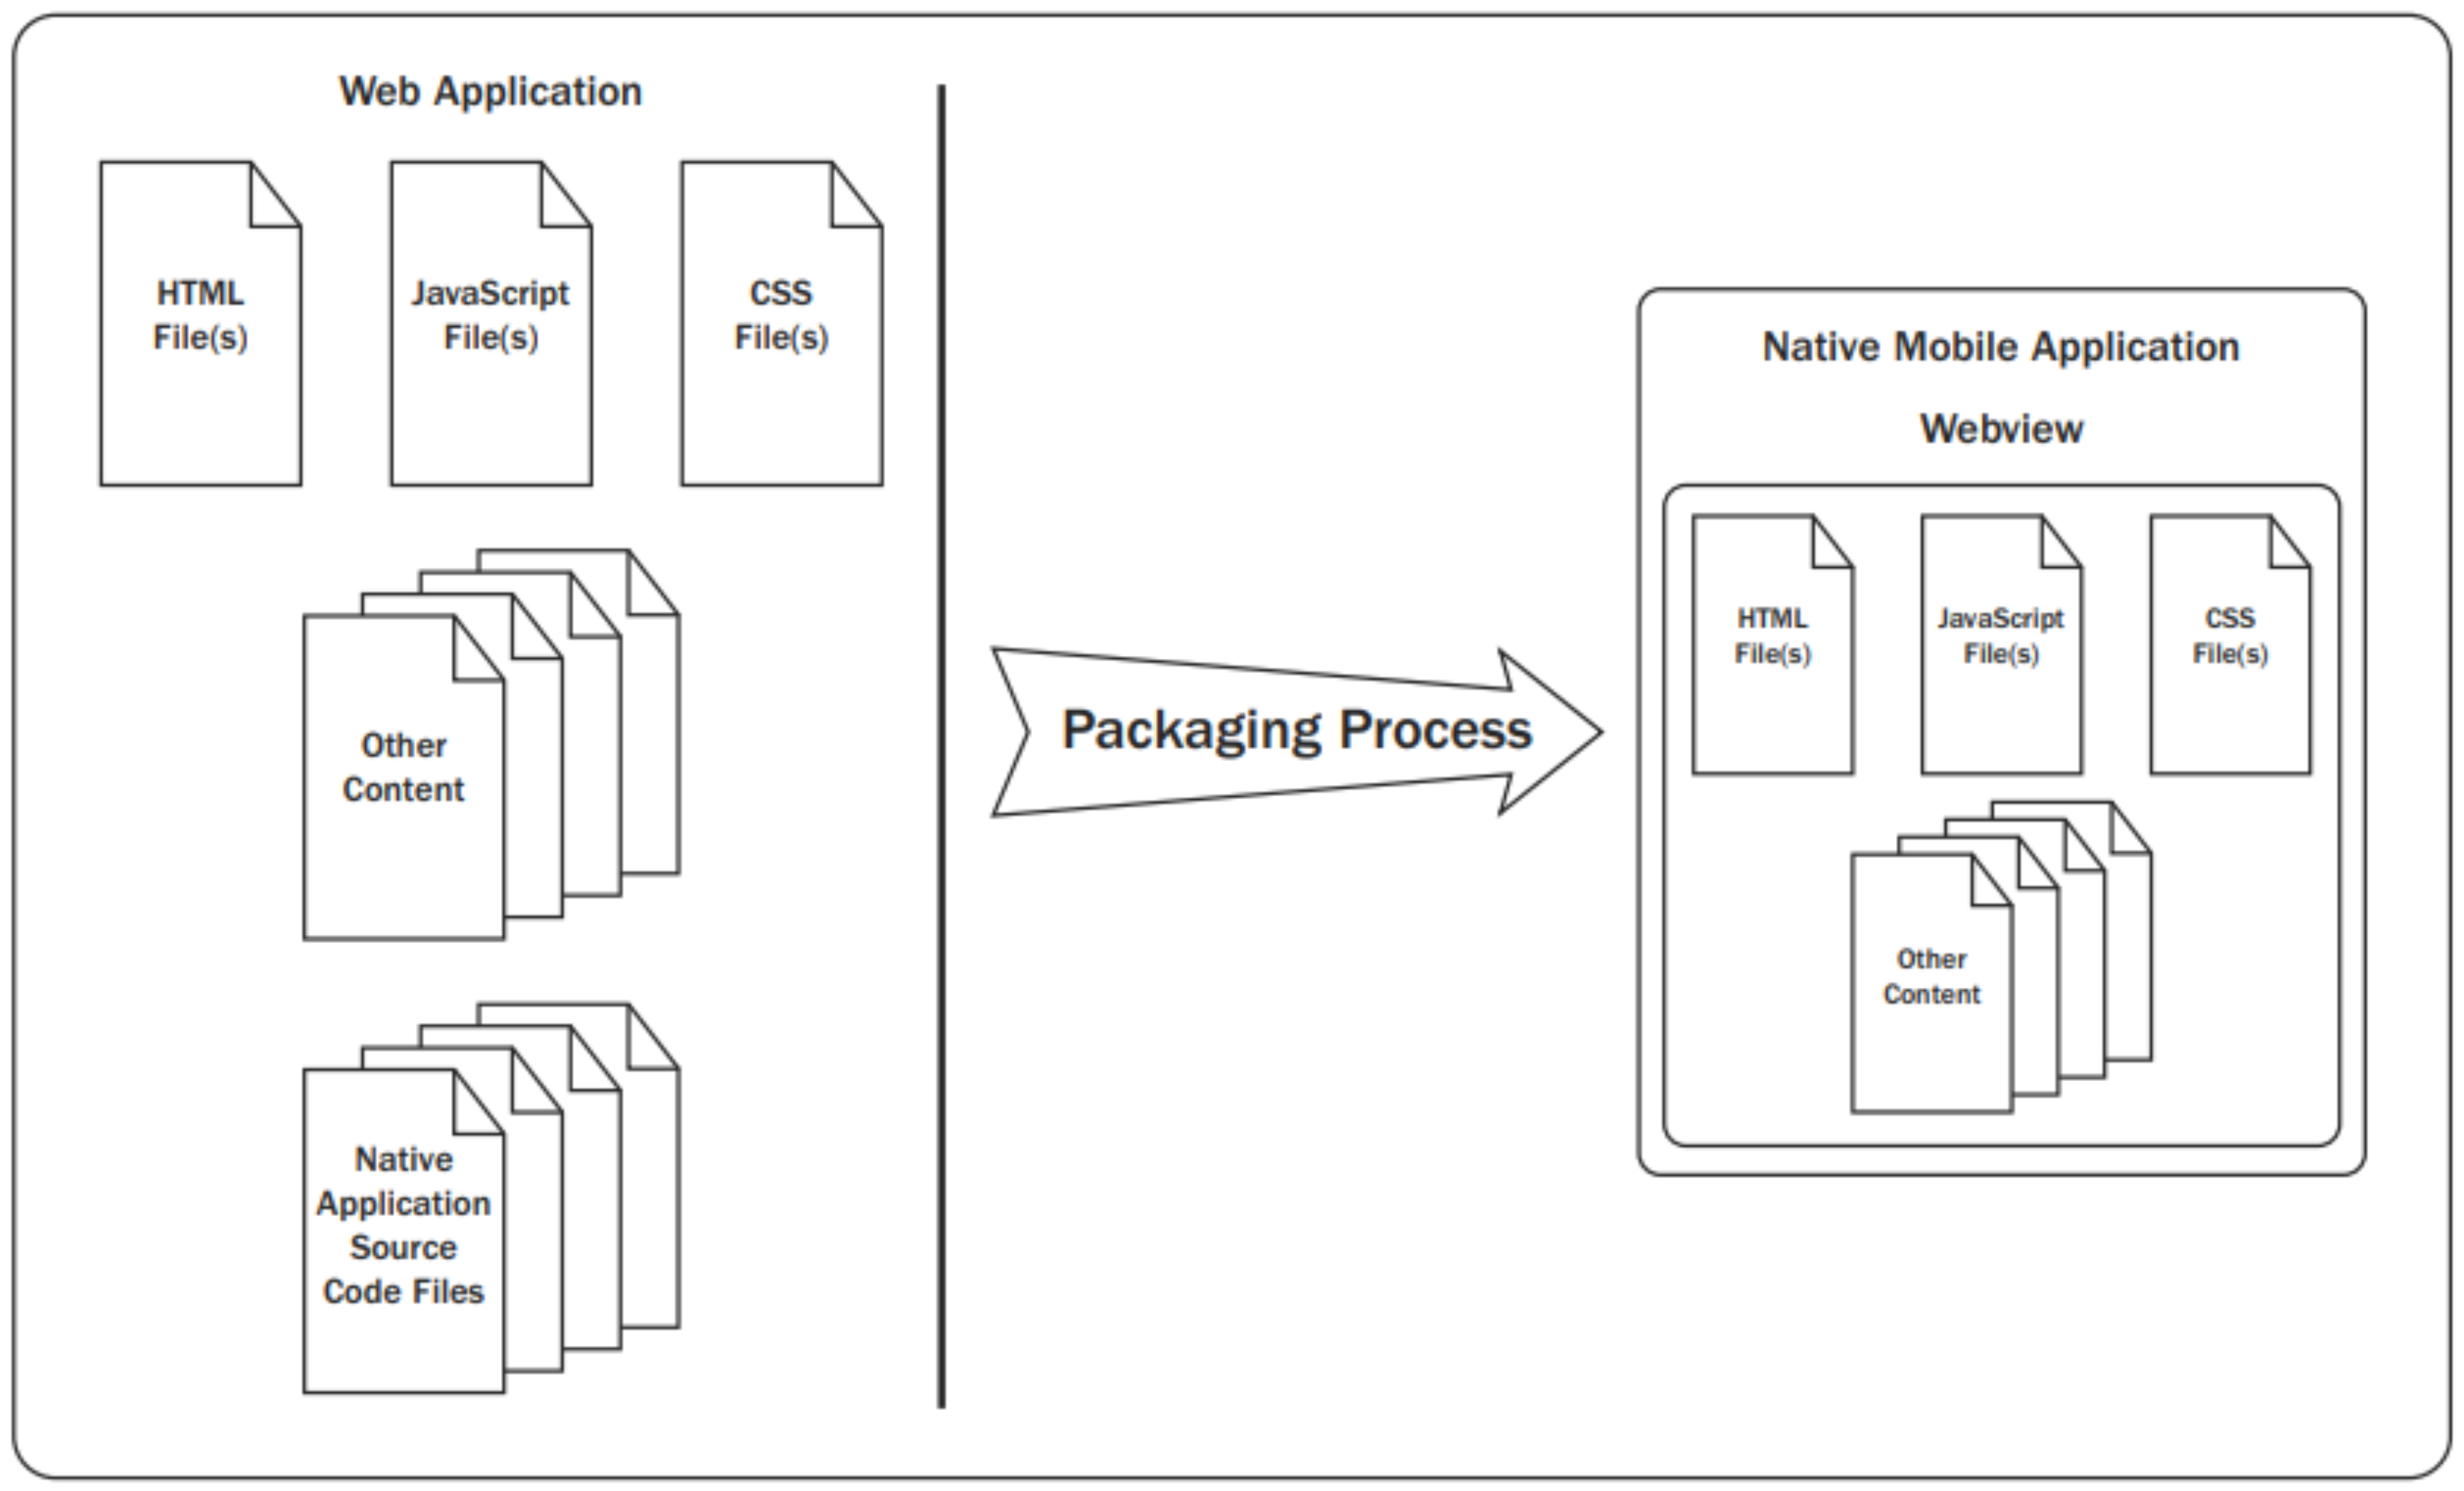
\includegraphics[scale=0.45]{Gambar/nativecontainercordova.png}
	    \caption{Proses Pengemasan Aplikasi Cordova~\cite{john:14:apache}}
	    \label{fig:nativecontainercordova}
\end{figure}

Di dalam aplikasi Cordova, antarmuka pengguna aplikasi terdiri dari satu layar yang hanya berisi satu tampilan web. Saat aplikasi dijalankan, aplikasi memuat halaman awal WebApp ke dalam tampilan web. WebApp yang berjalan di dalam \textit{native container} sama seperti aplikasi web lainnya yang berjalan di dalam browser web pada perangkat \textit{mobile}. WebApp dapat membuka halaman HTML, menjalankan logika JavaScript, dan mengimplementasi CSS, namun WebApp tidak dapat menjalankan fitur-fitur perangkat keras dan perangkat lunak dari perangkat \textit{mobile} seperti akselerometer, kamera, data kontak, dan fitur lainnya. Cordova menyediakan berbagai JavaScript API yang dapat digunakan agar aplikasi web yang berjalan di dalam \textit{native container} dapat mengakses kemampuan perangkat di luar kemampuan \textit{browser}. API ini diimplementasikan ke dalam JavaScript \textit{libraries} yang menjalankan fitur-fitur perangkat ke aplikasi web dengan implementasi yang disesuaikan dengan sistem operasi yang digunakan.

Cordova membuat aplikasi dapat mengakses fitur-fitur perangkat keras dan perangkat lunak suatu perangkat dengan menggunakan {\it plugin}. {\it Framework} Ionic~telah~terdapat~berbagai~macam~TypeScript~{\it wrapper}~untuk {\it plugins} Cordova.  Untuk dapat menggunakan Cordova Plugins, yaitu dengan memasang Cordova Plugins terlebih dahulu yang dapat dipasang dengan menjalankan Kode~\ref{lst:installCordova}, dan memperbaruinya ke versi terakhir pada Kode~\ref{lst:updateCordova} yang dapat dilakukan melalui CLI. Setiap {\it plugins} memiliki dua komponen, yaitu kode {\it native} (Cordova), dan kode TypeScript (Ionic Native).

\begin{lstlisting}[label={lst:installCordova}, caption=Kode untuk Memasang Cordova Plugins]
npm install cordova-plugin-name
npx cap sync
\end{lstlisting} 

\begin{lstlisting}[label={lst:updateCordova}, caption=Kode untuk Memperbarui Cordova Plugins]
npm install cordova-plugin-name@2
npx cap update
\end{lstlisting} 

\newpage

Sama seperti Capacitor, Cordova memiliki \textit{plugins} yang menyediakan antarmuka JavaScript ke komponen \textit{native}. Dengan menggunakan \textit{plugin} Cordova, aplikasi dapat menjalankan fitur-fitur perangkat \textit{mobile} seperti kamera,	geolokasi, dan file sistem. Salah satu \textit{plugin} yang tersedia yaitu Google Maps. \textit{Plugin} ini menghasilkan MapView secara \textit{native}, dan menempatkannya di bawah browser. MapView yang dihasilkan bukan merupakan HTMLElements, maka tidak terkait dengan HTML. Sebelum dapat menggunakan \textit{plugin} Google Maps, dilakukan instalasi \textit{plugin} untuk pertama kali pada \textit{command line}~\ref{lst:installGMapsCordova}. Selanjutnya atur Google Maps API Key di dalam \textit{file} config.xml~\ref{lst:apikeyGMapsCordova}. 

\begin{lstlisting}[label={lst:installGMapsCordova}, caption=Kode untuk Menginstal \textit{Plugin} Cordova Google Maps]
cordova plugin add cordova-plugin-googlemaps
\end{lstlisting} 

\begin{lstlisting}[label={lst:apikeyGMapsCordova}, caption=Kode untuk Mengatur API Key untuk \textit{Plugin} Cordova Google Maps]
<widget ...>
  <preference name="GOOGLE_MAPS_ANDROID_API_KEY" value="(api key)" />
  <preference name="GOOGLE_MAPS_IOS_API_KEY" value="(api key)" />
</widget>
\end{lstlisting} 

Cordova juga dapat menambahkan platform \textit{native} ke dalam proyek Ionic dengan mengetikan perintah seperti pada kode~\ref{lst:addCordovaAndroid} untuk menambahkan platform Android, dan kode~\ref{lst:addCordovaIOS} untuk menambahkan platform iOS. Untuk menjalankan proyek Ionic dengan Cordova dengan mengetikan perintah seperti pada kode~\ref{lst:runCordovaAndroid} untuk perangkat Android, dan kode~\ref{lst:runCordovaiOS} untuk perangkat iOS. Dengan begitu, Cordova akan membuka IDE sesuai dengan perintah yang dijalankan.

\begin{lstlisting}[label={lst:addCordovaAndroid}, caption=Kode untuk Menambahkan Platform Android dengan Cordova]
ionic cordova platform add android
\end{lstlisting} 

\begin{lstlisting}[label={lst:addCordovaIOS}, caption=Kode untuk Menambahkan Platform iOS dengan Cordova]
ionic cordova platform add iOS
\end{lstlisting} 

\begin{lstlisting}[label={lst:runCordovaAndroid}, caption=Kode untuk Membuat Aplikasi Cordova Untuk Perangkat Android]
ionic cordova platform run android
\end{lstlisting} 

\begin{lstlisting}[label={lst:runCordovaiOS}, caption=Kode untuk Membuat Aplikasi Cordova Untuk Perangkat iOS]
ionic cordova platform run iOS
\end{lstlisting} 

\subsection{UI Component}
\label{subsec:uiComponent}
{\it Framework} Ionic dapat menggunakan kemampuan Angular dalam memperluas kosakata HTML, yaitu menyertakan {\it tag} khusus untuk menciptakan seluruh rangkaian komponen~\cite{griffith:17:mobile}. Semua komponen memiliki awalan ion, sehingga dapat dikenali dalam markup. Sama seperti {\it tag} HTML standar, komponen Ionic juga dapat menerima berbagai macam atribut sebagai pengaturan dari {\it tag} tersebut, seperti mengatur id atau mendefinisikan kelas CSS tambahan. Terdapat beberapa komponen yang ada pada {\it framework} Ionic versi 6~[\ref{ref:uiComponents}]. Komponen-komponen tersebut yaitu:
\begin{itemize}
	\item Action Sheet \\
	Merupakan dialog yang menampilkan serangkaian opsi, yang muncul di atas konten aplikasi dan harus ditutup secara manual oleh pengguna sebelum pengguna dapat melanjutkan interaksi dengan aplikasi. Untuk menutup Action Sheet terdapat beberapa cara, termasuk mengetuk bagian selain Action Sheet atau menekan tombol escape di desktop.

	\item Alert \\
	Alert merupakan dialog yang menampilkan informasi kepada pengguna, atau mengumpulkan informasi dari pengguna menggunakan input. Alert muncul di atas konten aplikasi, dan harus ditutup secara manual oleh pengguna sebelum pengguna dapat melanjutkan interaksi dengan aplikasi. Secara opsional, terdapat header, sub header, dan pesan yang ada pada Alert.
	\item Badge \\
	Merupakan elemen {\it inline block} yang biasanya muncul di dekat elemen lain, berisi angka atau karakter lain, yang digunakan sebagai pemberitahuan bahwa ada item tambahan yang terkait dengan suatu elemen dan menunjukan berapa banyak item yang ada. Penggunaan Badge dengan menggunakan {\it tag} \texttt{<ion-badge>} (Kode~\ref{lst:badgeComponent}).
\begin{lstlisting}[label={lst:badgeComponent}, caption=Potongan Kode Program dari Badge Component]
<ion-badge>99</ion-badge>
\end{lstlisting} 
	\item Button \\
	Merupakan elemen yang dapat diklik, biasanya digunakan dalam formulir atau di mana pun yang membutuhkan fungsionalitas tombol. Button biasanya menampilkan teks, ikon, atau bisa juga keduanya. Button dapat pula menggunakan atribut untuk menampilkannya dengan penampilan tertentu. Penggunaan Button dengan menggunakan {\it tag} \texttt{<ion-button>} (Kode~\ref{lst:buttonComponent}). 
\begin{lstlisting}[label={lst:buttonComponent}, caption=Potongan Kode Program dari Button Component]
<ion-button>Default</ion-button>
\end{lstlisting} 

	\item Card \\
	Merupakan bagian standar dari tampilan antarmuka, yang tampak seperti kartu yang berfungsi sebagai titik masuk ke dalam informasi yang lebih detail. Card dapat menjadi satu komponen, tetapi sering kali terdiri dari beberapa header, judul, sub judul, dan konten. Penggunaan Card dengan menggunakan {\it tag} \texttt{<ion-card>} yang dapat berisi {\it header}, {\it subtitle}, {\it title}, dan {\it content} (Kode~\ref{lst:cardComponent}).

\begin{lstlisting}[label={lst:cardComponent}, caption=Potongan Kode Program dari Card Component]
<ion-card>
	<ion-card-header>
		<ion-card-subtitle>Card Subtitle</ion-card-subtitle>
		<ion-card-title>Card Title</ion-card-title>
	</ion-card-header>
				
	<ion-card-content>
		Card Content
	</ion-card-content>
</ion-card>
\end{lstlisting} 
	
	\item Content\\
	Komponen content merupakan penyedia area konten yang bisa digunakan untuk mengontrol area yang dapat digulir. Dalam satu tampilan, setidaknya terdapat satu buah content. Content juga dapat dimodifikasi padding, margin, dan lainnya menggunakan {\it global style} yang berada di CSS Utilites atau mengubahnya secara individual dengan menggunakan CSS. Penggunaan Content dengan menggunakan {\it tag} \texttt{<ion-content>} (Kode~\ref{lst:contentComponent}).

\begin{lstlisting}[label={lst:contentComponent}, caption=Potongan Kode Program dari Content Component]
<ion-content
	[scrollEvents]="true"
	(ionScrollStart)="logScrollStart()"
	(ionScroll)="logScrolling($event)"
	(ionScrollEnd)="logScrollEnd()">
		<h1>Main Content</h1>
			
			<div slot="fixed">
				<h1>Fixed Content</h1>
			</div>
</ion-content>
\end{lstlisting} 

	\item Date and Time Pickers\\
	Datetime merupakan penampil antarmuka untuk pengguna memilih tanggal dan waktu. Terdapat kolom yang dapat digulir yang dapat digunakan untuk memilih tahun, bulan, hari, jam, dan menit secara individual. Komponen ini menampilkan nilai di dua tempat, yaitu di komponen \texttt{<ion-datetime>} (Kode~\ref{lst:datetimeComponent}), dan di antarmuka pemilih yang ditampilkan dari bawah layar.
\begin{lstlisting}[label={lst:datetimeComponent}, caption=Kode Program dari Datetime Component dengan Format Bulan-Hari-Tahun]
<ion-datetime displayFormat="MM DD YY" placeholder="Select Date"></ion-datetime>
\end{lstlisting} 

	\item Grid \\
	Grid digunakan untuk membuat tata letak kustom pada tampilan. Grid terdiri dari tiga bagian, yaitu \textit{grid}, baris, dan kolom. Masing-masing kolom dapat diubah ukurannya menggunakan CSS. Grid digunakan dengan \textit{tag} \texttt{<ion-grid>} (Kode~\ref{lst:GridComponent}).	

\begin{lstlisting}[label={lst:GridComponent}, caption=Potongan Kode Program dari Grid Component]
<ion-row>
	<ion-col size="6">
    	ion-col [size="6"]
    </ion-col>
    <ion-col>
      	ion-col
    </ion-col>
</ion-row>
\end{lstlisting}
	\newpage
	\item Infinite Scroll	\\
	Komponen Infinite Scroll memanggil sebuah action yang akan dilakukan ketika pengguna menggulir dengan jarak tertentu dari bawah atau atas halaman. Penggunaan Infinite Scroll dengan menggunakan {\it tag} \texttt{<ion-infinite-scroll>} (Kode~\ref{lst:InfiteScrollComponent}). 
	
\begin{lstlisting}[label={lst:InfiteScrollComponent}, caption=Potongan Kode Program dari Infinite Scroll Component]
<ion-infinite-scroll threshold="100px" (ionInfinite)="loadData($event)">
	<ion-infinite-scroll-content
		loadingSpinner="bubbles"
		loadingText="Loading more data...">
	</ion-infinite-scroll-content>
</ion-infinite-scroll>
\end{lstlisting}
	
	\item Icon \\
	Icon merupakan komponen yang berupa gambar kecil, yang merepresentasikan sebuah berkas, dan folder di dalam aplikasi. Penggunaan Icon adalah dengan menggunakan {\it tag} \texttt{<ion-icon>} (Kode~\ref{lst:iconComponent}).
\begin{lstlisting}[label={lst:iconComponent}, caption=Potongan Kode Program dari Icon Home]
<ion-icon name="home"></ion-icon>
\end{lstlisting} 
	\item Item \\
	Item merupakan elemen yang dapat berisi teks, ikon, avatar, gambar, masukan, dan elemen asli atau kustom lainnya. Biasanya, item ditempatkan di dalam sebuah {\it list} bersamaan dengan item lainnya dengan {\it tag} \texttt{<ion-item>} (Kode~\ref{lst:itemComponent}). Dapat dilakukan {\it swipe}, dihapus, disusun ulang, dan diedit.
	
\begin{lstlisting}[label={lst:itemComponent}, caption=Potongan Kode Program dari Item Component]
<ion-item>
	<ion-label>
		Item
	</ion-label>
</ion-item>
\end{lstlisting} 
	
	\item List \\
	Komponen List terdiri dari beberapa baris \textit{item} yang dapat berisi teks, tombol, \textit{toggles}, ikon, thumbnails, dan komponen-komponen lainnya menggunakan \textit{tag} \texttt{<ion-list>} (Kode~\ref{lst:listComponent}). List mendukung untuk pengguna melakukan \textit{swiping}, \textit{dragging}, dan penghapusan \textit{item}. 
	
\begin{lstlisting}[label={lst:listComponent}, caption=Potongan Kode Program dari List Component]
<ion-list>
  <ion-item>
    <ion-label>Pokemon Yellow</ion-label>
  </ion-item>
  <ion-item>
    <ion-label>Mega Man X</ion-label>
  </ion-item>
  <ion-item>
    <ion-label>The Legend of Zelda</ion-label>
  </ion-item>
  <ion-item>
    <ion-label>Pac-Man</ion-label>
  </ion-item>
  <ion-item>
    <ion-label>Super Mario World</ion-label>
  </ion-item>
</ion-list>
\end{lstlisting} 		
	
	\item Menu \\
	Komponen Menu merupakan panel navigasi samping yang dapat dilakukan {\it slides} dari sisi pada tampilan halaman saat ini menggunakan {\it tag} \texttt{<ion-menu>} (Kode~\ref{lst:menuComponent}). Pada dasarnya, Menu muncul dari kiri, tetapi sisi kemunculan menu dapat diganti. 

\begin{lstlisting}[label={lst:menuComponent}, caption=Potongan Kode Program dari Menu Component]
<ion-menu side="start" menuId="first" contentId="main">
	<ion-header>
		<ion-toolbar color="primary">
			<ion-title>Start Menu</ion-title>
		</ion-toolbar>
	</ion-header>
	<ion-content>
		<ion-list>
			<ion-item>Menu Item</ion-item>
			<ion-item>Menu Item</ion-item>
			<ion-item>Menu Item</ion-item>
			<ion-item>Menu Item</ion-item>
			<ion-item>Menu Item</ion-item>
		</ion-list>
	</ion-content>
</ion-menu>
\end{lstlisting} 
	\item Modal \\
	Modal merupakan kotak dialog yang muncul diatas konten aplikasi lain, dan harus diutup secara manual oleh pengguna sebelum pengguna dapat melanjutkan menggunakan aplikasi. Modal berguna sebagai komponen pilihan ketika ada banyak opsi untuk dipilih, atau melakukan penyaringan isi di dalam daftar, serta beberapa kasus serupa lainnya. Modal dapat digunakan dengan \textit{tag} \texttt{<ion-modal>} (Kode~\ref{lst:modalComponent}).

\begin{lstlisting}[label={lst:modalComponent}, caption=Kode Program dari Modal]
<ion-modal [isOpen]="true">
  <ng-template>
    <ion-content>Modal Content</ion-content>
  </ng-template>
</ion-modal>
\end{lstlisting} 

\newpage

	\item Navigation \\
	Navigation adalah komponen mandiri yang digunakan untuk membuat komponen baru ke dalam {\it stack}. Navigation tidak terikat kepada {\it router} tertentu, mengakibatkan jika kita membuat komponen Navigation dan melakukan {\it push} komponen lain ke dalam {\it stack}, komponen tersebut tidak akan mempengaruhi router aplikasi secara keseluruhan. Sesuai dengan kasus penggunaan dimana ketika pengguna bisa memilih modal, yang membutuhkan sub-navigasinya sendiri, tanpa membuatnya terikat ke URL aplikasi. 
	
	\item Refresher \\
	Refresher merupakan komponen yang menyediakan fungsionalitas \textit{pull-to-refresh} pada komponen konten dengan \textit{tag} \texttt{<ion-refresher>} (Kode~\ref{lst:refresherComponent}). Refresher digunakan pada saat pengguna menarik layar dari atas ke bawah, maka Refresher akan menyegarkan data atau mendapatkan daftar data untuk mengambil lebih banyak data. 
	
\begin{lstlisting}[label={lst:refresherComponent}, caption=Kode Program dari Refresher]
<ion-content>
  <ion-refresher slot="fixed" (ionRefresh)="doRefresh($event)">
    <ion-refresher-content></ion-refresher-content>
  </ion-refresher>
</ion-content>
\end{lstlisting}
	\item Segment \\
	Segment berfungsi untuk menampilkan pilihan tombol bagi pengguna untuk beralih di antara tampilan berbeda di dalam satu halaman yang sama. Segment menampilkan sekelompok tombol-tombol yang dapat diklik, dalam baris horizontal. Penggunaan Segment dengan menggunakan {\it tag} \texttt{<ion-segment>} (Kode~\ref{lst:segmentComponent}).
	
\begin{lstlisting}[label={lst:segmentComponent}, caption=Kode Program dari Segment]
<ion-segment (ionChange)="segmentChanged($event)">
	<ion-segment-button value="friends">
		<ion-label>Friends</ion-label>
	</ion-segment-button>
	<ion-segment-button value="enemies">
		<ion-label>Enemies</ion-label>
	</ion-segment-button>
</ion-segment>
\end{lstlisting}
	
	\item Slides \\
	Komponen Slides merupakan sebuah \textit{multi-section container} yang setiap bagiannya dapat dilakukan \textit{swipe} atau \textit{drag}. Untuk menggunakan komponen ini dengan menggunakan \textit{tag} \texttt{<ion-slides>} seperti pada kode~\ref{lst:slidesComponent} sebagai pembungkus slide. Masing-masing slide menggunakan \textit{tag} \texttt{<ion-slide>} seperti pada baris ke-2. \textit{Tag} tersebut dapat digunakan untuk menggeser slide dari kiri ke kanan, atau sebaliknya.

\newpage	
	
\begin{lstlisting}[label={lst:slidesComponent}, caption=Kode Program dari Slides]
<ion-slides pager="true" [options]="slideOpts">
	<ion-slide>
		<h1>Slide 1</h1>
	</ion-slide>
	<ion-slide>
		<h1>Slide 2</h1>
	</ion-slide>
	<ion-slide>
		<h1>Slide 3</h1>
	</ion-slide>
</ion-slides>
\end{lstlisting}
	
	\item Tabs \\
	Tabs merupakan navigasi {\it top-level} yang mengimplementasi sebuah {\it tab-based navigation}. Tabs dapat digunakan dengan {\it tag} \texttt{<ion-tabs>} (Kode~\ref{lst:tabsComponent}) yang tidak memliki {\it styling} apapun dan bekerja sebagai {\it router outlet} untuk menangani navigasi. 
\begin{lstlisting}[label={lst:tabsComponent}, caption=Kode Program dari Tabs]
<ion-tabs>
	<ion-tab-bar slot="bottom">
		<ion-tab-button tab="schedule">
			<ion-icon name="calendar"></ion-icon>
			<ion-label>Schedule</ion-label>
			<ion-badge>6</ion-badge>
		</ion-tab-button>

		<ion-tab-button tab="speakers">
			<ion-icon name="person-circle"></ion-icon>
			<ion-label>Speakers</ion-label>
		</ion-tab-button>
	</ion-tab-bar>
</ion-tabs>
\end{lstlisting}
		
	\item Toast \\
	Komponen Toast merupakan sebuah notifikasi yang digunakan di aplikasi modern untuk memberikan umpan balik atau menampilkan pesan sistem. Komponen ini muncul diatas konten aplikasi, dan dapat ditutup untuk melanjutkan penggunaan aplikasi. Komponen ini menggunakan ToastController yang dimiliki oleh \textit{library} Ionic Angular (Kode~\ref{lst:toastComponent}) 

\begin{lstlisting}[label={lst:toastComponent}, caption=Kode Program dari Toast]
async presentToast() {
    const toast = await this.toastController.create({
      message: 'Your settings have been saved.',
      duration: 2000
    });
    toast.present();
}
\end{lstlisting}
		

	\item Toolbar \\
	Toolbar dapat diposisikan di atas ataupun di bawah konten. Ketika toolbar ditempatkan di header \texttt{<ion-header>} akan muncul di bagian atas konten, sedangkan ketika ditempatkan di footer \texttt{<ion-footer>} akan muncul tetap di bagian bawah. Toolbar menggunakan {\it tag} \texttt{<ion-toolbar>}, yang di dalamnya dapat berisi button, dan dapat menggunakan border (Kode~\ref{lst:datetimeComponent}).

\begin{lstlisting}[label={lst:datetimeComponent}, caption=Kode Program dari Toolbar dengan Button di Dalamnya]
<ion-toolbar>
	<ion-buttons slot="start">
		<ion-back-button></ion-back-button>
	</ion-buttons>
	<ion-title>Back Button</ion-title>
</ion-toolbar>
\end{lstlisting} 
\end{itemize}
	Selain komponen-komponen yang telah disebutkan, tertapat beberapa komponen lainnya yang tidak disebutkan disini. Komponen-komponen tersebut yaitu Checkbox, Chip, Floating Action Button, Grid, Input, Popover, Progress Indicator, Radio, Reorder, Routing, Searchbar, Select, dan Toggle~\footnote{\textit{`UI Components'} https://ionicframework.com/docs/components, Diakses pada 17 April 2022. \label{ref:uiComponents}}.
%2.2.1 Native API
%2.2.1.1 Capacitor
%2.2.1.2 Cordova
%2.2.2 UI Component 

\subsection{Migrasi Ionic 3 ke Ionic 6}
\label{subsec:migrasi}
%Aplikasi WSDC Bali 2017 saat ini menggunakan {\it framework} Ionic versi 3 yang sudah tidak didukung lagi. Maka dari itu dilakukan pembaruan aplikasi WSDC 2017 Bali ke dalam {\it framework} Ionic versi 5. 

Untuk melakukan migrasi dari Ionic 3 ke Ionic 6 memerlukan tiga tahap, yaitu migrasi dari Ionic 3 ke Ionic 4, migrasi Ionic 4 ke Ionic 5, dan migrasi dari Ionic 5 ke Ionic 6. Tahapan migrasi tersebut adalah sebagai berikut:

%---START ENUM SECTION MIGRASI IONIC 3 KE IONIC 5---%
\begin{enumerate}
	\item Migrasi Ionic 3 ke Ionic 4 \\
	Ada beberapa langkah untuk melakukan migrasi dari Ionic 3 ke dalam Ionic 4, yaitu:
	

	%---START ENUM MIGRASI IONIC 3 KE IONIC 4---%
	\begin{enumerate}
		\item Membuat Proyek Ionic Baru \\
		Untuk membuat projek Ionic baru tanpa {\it template} apapun dengan menggunakan perintah \textbf{ionic start myApp blank} dan memilih Angular sebagai {\it framework}nya~\ref{lst:createNewProject}.
\begin{lstlisting}[label={lst:createNewProject}, caption=Perintah Membuat Proyek Ionic Baru]
ionic start myApp blank
\end{lstlisting}

		\item Menyalin Angular Services yang pada Ionic 3 berada di \textbf{src/providers}, menjadi \textbf{src/app/services} pada Ionic 4.

		\item Menyalin {\it Root-level Items} \\
		Menyalin seluruh {\it Root-level Items} pada Ionic versi 3, seperti \textit{pipes} dan \textit{components}. Terdapat perubahan struktur direktori dengan perubahan direktori yang semula \textbf{src/components} pada Ionic 3, menjadi \textbf{src/app/components} pada Ionic 4.

		\item Menyalin Global Scss dari \textbf{src/app/app.scss} pada Ionic 3, menjadi \textbf{src/global.scss} pada Ionic 4.

		\item Menyalin Bagian-bagian Aplikasi \\
		Menyalin keseluruhan bagian yang ada pada aplikasi, baik itu halaman maupun fitur yang ada, dengan ketentuan sebagai berikut :

		%---START ITEMIZE MENYALIN BAGIAN BAGIAN APLIKASi---%
		\begin{itemize}
			\item Shadow DOM sudah aktif secara {\it default}.
			\item Page atau Components Sass tidak lagi dibungkus dengan \textit{tag page} atau \textit{components} dan harus menggunakan opsi styleUrls milik Angular dari dekorator @Component.
			\item Perubahan RxJS yang digunakan. Pada ionic 3 adalah versi 5, sedangkan pada Ionic 4 RxJS yang digunakan adalah versi 6.
			\item Lifecycle Hooks tertentu harus digantikan dengan Angular Hooks.
			\item Perubahan markup yang mungkin saja dibutuhkan. \\
			Sejak Ionic 4 dipindahkan ke elemen kustom, terdapat perubahan yang signifikan terkait dengan markup untuk setiap komponen. Semua perubahan ini dibuat untuk mengikuti spesifikasi dari elemen kustom. Komponen-komponen yang berubah tersebut yaitu :

			\begin{itemize}
				\item {\it Button} \\
				Terdapat perbedaan pada {\it tag} untuk membuat Button, yang semula pada Ionic 3 adalah \texttt{<button>} menjadi \texttt{<ion-button>} pada Ionic 4 (Kode~\ref{lst:buttonIonic4}).
\begin{lstlisting}[label={lst:buttonIonic4}, caption=Penggunaan Button pada Ionic 4]
<ion-button (click)="doSomething()">
	Default Button
</ion-button>
\end{lstlisting}

				\item Floating Action Button (FAB) \\
				Terdapat perbedaan pada {\it tag} di dalam \texttt{<ion-fab>}, yang semula pada Ionic 3 adalah \texttt{<button>} menjadi \texttt{<ion-fab-button>} pada Ionic 4 (Kode~\ref{lst:fabIonic4}).

\begin{lstlisting}[label={lst:fabIonic4}, caption=Penggunaan Floating Action Button pada Ionic 4]
<ion-fab>
	<ion-fab-button>
		<ion-icon name="add"></ion-icon>
	</ion-fab-button>
	<ion-fab-list>
		<ion-fab-button>
			<ion-icon name="logo-facebook"></ion-icon>
		</ion-fab-button>
	</ion-fab-list>
</ion-fab>
\end{lstlisting}
				
				\item Item \\
				Terdapat perbedaan pada \textit{tag} \texttt{<ion-item>}, dimana pada Ionic 3, \textit{tag} \texttt{<ion-label>} akan secara otomatis ditambahkan ke dalam \texttt{<ion-item>}. Sedangkan pada Ionic 4 diharuskan untuk menambahkan \textit{tag} \texttt{<ion-label>} secara manual ke dalam komponen item (Kode~\ref{lst:itemIonic4}). 
				
\begin{lstlisting}[label={lst:itemIonic4}, caption=Penggunaan Item pada Ionic 4]
<ion-item>
	<ion-label>
    	Default Item
	</ion-label>
</ion-item>
\end{lstlisting}

				\item Label \\
				Pada Ionic 4, atribut untuk mengatur posisi dari label digabungkan dengan atribut {\it position} (Kode~\ref{lst:atributIonic4}).
\begin{lstlisting}[label={lst:atributIonic4}, caption=Penggunaan Atribut {\it Position} pada Ionic 4]
<ion-item>
	<ion-label position="floating">Floating Label</ion-label>
	<!-- input -->
</ion-item>
\end{lstlisting}

				\item Menu \\
				Terdapat beberapa perubahan nama pada Ionic 4, yaitu:
				\begin{itemize}
					\item Perubahan Nama Properti
					Terdapat perubahan nama properti pada Ionic 4. Perubahan-perubahan tersebut adalah sebagai berikut:
\begin{table}[H]
\centering
\begin{tabular}{|p{4cm}|p{4cm}|p{4cm}|}
  \hline
  \multicolumn{1}{|c|}{\multirow{2}{*}{Properti}} & \multicolumn{2}{c|}{Perubahan}                   \\ \cline{2-3} 
                               					  & Ionic 3 & Ionic 4 \\ \hline
	swipeEnabled                                  & swipeEnabled & swipeGesture \\ \hline
    content                                     & content     & contentId    \\ \hline
\end{tabular}
\end{table}			

					\item Perubahan Nama Events
					Terdapat perubahan nama {\it events} pada Ionic 4. Perubahan-perubahan tersebut adalah sebagai berikut :
					
\begin{table}[H]
\centering
\begin{tabular}{|p{4cm}|p{4cm}|p{4cm}|}
  \hline
  \multicolumn{1}{|c|}{\multirow{2}{*}{Events}}   & \multicolumn{2}{c|}{Perubahan}                   \\ \cline{2-3} 
                               					  & Ionic 3      & Ionic 4 \\ \hline
	ionClose                                      & ionClose     & ionDidClose \\ \hline
    ionOpen                                       & ionOpen      & ionDidOpen    \\ \hline
\end{tabular}
\end{table}		
				\end{itemize}

				\item Nav \\
				Terdapat perubahan Nav pada Ionic 4. Perubahan-perubahan tersebut adalah sebagai berikut:
				\begin{itemize}
					\item Perubahan Nama Method 
					Terdapat perubahan nama {\it method} pada Ionic 4. Perubahan-perubahan tersebut adalah sebagai berikut:

\begin{table}[H]
\centering
\begin{tabular}{|p{4cm}|p{4cm}|p{4cm}|}
  \hline
  \multicolumn{1}{|c|}{\multirow{2}{*}{Nama Method}}   & \multicolumn{2}{c|}{Perubahan}                   \\ \cline{2-3} 
                               					       & Ionic 3                 & Ionic 4 \\ \hline
	remove                                             & remove                  & getChildNavs \\ \hline
    getActiveChildNavs                                 & getActiveChildNavs      & getChildNavs    \\ \hline
\end{tabular}
\end{table}				

					\item Perubahan Nama Prop \\
					Terdapat perubahan nama prop pada Ionic 4. Perubahan tersebut adalah sebagai berikut:\\

\begin{table}[H]
\centering
\begin{tabular}{|p{4cm}|p{4cm}|p{4cm}|}
  \hline
  \multicolumn{1}{|c|}{\multirow{2}{*}{Nama Prop}}     & \multicolumn{2}{c|}{Perubahan}                   \\ \cline{2-3} 
                               					       & Ionic 3                 & Ionic 4 \\ \hline
	swipeBackEnabled                                   & swipeBackEnabled        & swipeGesture \\ \hline
\end{tabular}
\end{table}		
				\end{itemize}	
\newpage
				\item Navbar \\
				Pada Ionic 4, terdapat penghapusan terhadap komponen \texttt{<ion-navbar>} karena untuk menjaga agar selalu menggunakan \texttt{<ion-toolbar>} dengan {\it back button} yang eksplisit (Kode~\ref{lst:navbarIonic4}).				
				
\begin{lstlisting}[label={lst:navbarIonic4}, caption=Penggunaan Navbar pada Ionic 4 dengan {\it Back Button}]
<ion-toolbar>
	<ion-buttons slot="start">
		<ion-back-button></ion-back-button>
	</ion-buttons>
	<ion-title>My Navigation Bar</ion-title>
</ion-toolbar>
\end{lstlisting}
				
				\item Overlays \\
				Pada Ionic 4, semua overlay harus menggunakan async/await. Overlay tersebut adalah Action Sheet, Alert, Loading, Modal, Popover, and Toast (Kode~\ref{lst:overlaysIonic4}). Terjadi perubahan nama properti enableBackdropDismiss menjadi backdropDismiss.
				
\begin{lstlisting}[label={lst:overlaysIonic4}, caption=Penggunaan Overlay untuk Toast pada Ionic 4]
async presentToast() {
    const toast = await this.toastController.create({
      message: 'Your settings have been saved.',
      duration: 2000
    });
    toast.present();
}
\end{lstlisting}
				
				\item Scroll \\
				\textit{Tag} \texttt{<ion-scroll>} sudah dihapus pada Ionic 4 agar penggunaan \textit{tag} \texttt{<ion-content>} menjadi lebih maksimal.
				
				\item Segment Button \\
				Pada Ionic 4, teks pada Segment Button membutuhkan \texttt{<ion-label>} untuk membungkusnya (Kode~\ref{lst:segmentButtonIonic4}).
\begin{lstlisting}[label={lst:segmentButtonIonic4}, caption=Penggunaan Segment Button untuk Toast pada Ionic 4]
<ion-segment-button>
	<ion-label>Item One</ion-label>
</ion-segment-button>
\end{lstlisting}
				
			\end{itemize}

			Selain yang telah disebutkan, terdapat beberapa perubahan lainnya yang tidak ditulis seperti Action Sheet, Alert, Colors, Content, Datetime, Dynamic Mode, Fixed Content, Grid, Icon, Infinite Scroll, Item Divider, Item Options, Item Sliding, List Header, Loading, Modal, Option, Popover, Radio, Range, Refresher, Select, Show When, Hide When, Spinner, Tabs, Typography, Therming, dan Toolbar~\footnote{\textit{`Breaking Changes'} https://github.com/ionic-team/ionic-framework/blob/main/angular/BREAKING.md, Diakses pada 13 November 2021. \label{ref:breakingChanges}}.
		\end{itemize}
		%---END ITEMIZE MENYALIN BAGIAN BAGIAN APLIKASi---%


	\end{enumerate}
	%---END ENUM MIGRASI IONIC 3 KE IONIC 4---%
	\item Migrasi Ionic 4 ke Ionic 5 \\
	Migrasi aplikasi dari Ionic 4 ke Ionic 5 memerlukan beberapa pembaruan mengenai properti API, CSS, dan {\it package dependencies} yang terpasang. Perubahan-perubahan tersebut yaitu :

	%---START ITEMIZE MIGRASI IONIC 4 KE IONIC 5---%
	\begin{itemize}
		\item CSS
		\begin{itemize}
			\item {\it Activated, Focused, Hover States} \\
			Kelas .activated secara otomatis ditambahkan ke komponen yang dapat diklik, mengalami perubahan nama menjadi .ion-activated. Terdapat pembaruan komponen Action Sheet sehingga variabel akan diawali dengan {\it button}. Hal ini dapat memungkinkan aplikasi tetap memiliki kontrol atas {\it opacity} jika diinginkan, tetapi saat memperbarui status, hanya perlu mengatur variabel utama, yaitu -background-activated, -background-focused, -background-hover. Hal tersebut penting saat mengubah tema global, karena memperbarui warna {\it toolbar} akan secara otomatis memperbarui {\it hover states} untuk semua {\it buttons} di {\it toolbar} (Kode~\ref{lst:hoverStates}). 		
			
\begin{lstlisting}[label={lst:hoverStates}, caption=Contoh Kode {\it Hover States} pada Ionic 5]
/* Setting the button background on hover to solid red */
ion-button {
	--background-hover: red;
	--background-hover-opacity: 1;
}

/* Setting the action sheet button background on focus to an opaque green */
ion-action-sheet {
	--button-background-focus: green;
	--button-background-focus-opacity: 0.5;
}

/*
* Setting the fab button background on hover to match the text color with
* the default --background-hover-opacity on md
*/
.md ion-fab-button {
	--color: #222;
	--background-hover: #222;
}
\end{lstlisting} 

			\item CSS {\it Utilities} \\
			Karena pada versi sebelumnya, yaitu Ionic versi 4, terdapat masalah dengan menggunakan atribut CSS dengan {\it framework} yang menggunakan JSX dan TypeScript, Ionic {\it Framework} menambahkan dukungan untuk beberapa {\it framework}, dan pada Ionic 5 menambahkan kelas CSS. Ionic versi 5 menghapus atribut CSS dan mendukung konsistensi. Ionic versi 5 juga mengubah ke kelas dengan diawali ion untuk menghindari konflik dengan atribut asli dan CSS dari pengguna (Kode~\ref{lst:CSSUtilities}).		
			
\begin{lstlisting}[label={lst:CSSUtilities}, caption=Contoh Kode Kelas CSS {\it Utility} pada Ionic 5]
<ion-header class="ion-text-center"></ion-header>
<ion-content class="ion-padding"></ion-content>
<ion-label class="ion-text-wrap"></ion-label>
<ion-item class="ion-wrap"></ion-item>
\end{lstlisting} 
  \newpage
			\item {\it Display Classes} \\ 
			Kelas dari {\it responsive display} yang ditemukan di dalam berkas display.css memiliki kueri media yang diperbarui untuk lebih mencerminkan bagaimana cara kerjanya.

			\item {\it Distributed Scss} \\
			Berkas scss telah dihapus dari dist/. Sebagai gantinya, variabel CSS harus digunakan untuk tema.

		\end{itemize}

		\item Komponen\\
		Terdapat perubahan beberapa komponen pada Ionic 5, yaitu :
		\begin{itemize}
			\item Back Button dan Button  \\
			Perubahan terdapat pada penambahan penamaan kelas .activated yang secara otomatis ditambahkan ke komponen yang dapat di klik, menjadi .ion-activated.
			
			\item Controllers\\
			Terdapat beberapa komponen yang dihapus dari Ionic sebagai elemen, yaitu ion-action-sheet-controller, ion-alert-controller, ion-loading-controller, ion-menu-controller, ion-modal-controller, ion-picker-controller, ion-popover-controller, dan ion- toast-controller. Sebagai gantinya, maka harus diimpor dari @ionic/core. 
			\item Header dan Footer\\
			Atribut no-border dihapus, dan sebagai gantinya yaitu dengan menggunakan kelas ion-no-border.
			
			\item List Header\\
			Konten berupa teks apa pun di dalam \texttt{<ion-list-header>} harus dibungkus dengan \texttt{<ion-label>} sesuai dengan gaya desain yang baru (Kode~\ref{lst:listHeader}). Jika label tidak ada, maka perataan tombol di header bisa saja terlihat tidak aktif. 

\begin{lstlisting}[label={lst:listHeader}, caption=Kode Program untuk List Header]
<ion-list-header>
	<ion-label>New This Week</ion-label>
	<ion-button>See All</ion-button>
</ion-list-header>
\end{lstlisting}
			\item Menu\\
			Fungsi swipeEnable() telah dihapus di Angular, sebagai gantinya menggunakan swipeGesture(). Nilai {\it left} dan {\it right} telah dihapus, dan menggunakan {\it start} dan {\it end} sebagai gantinya. Terdapat penghapusan atribut utama, sebagai gantinya yaitu dengan menggunakan content-id (untuk vanila JS atau Vue) dan contentId (untuk Angular atau React) (Kode~\ref{lst:menu}).			
			
\begin{lstlisting}[label={lst:menu}, caption=Kode Program untuk Menu]
<ion-menu content-id="main"></ion-menu>
<ion-content id="main">...</ion-content>
\end{lstlisting}

\newpage
			\item Select Option \\
			Properti selected telah dihapus. Sebagai gantinya harus mengatur properti nilai pada ion-select induk agar sesuai dengan opsi terpilih yang diinginkan (Kode~\ref{lst:selectOption}).
\begin{lstlisting}[label={lst:selectOption}, caption=Kode Program untuk Select Option]
<ion-select value="two">
	<ion-select-option value="one">One</ion-select-option>
	<ion-select-option value="two">Two</ion-select-option>
</ion-select>
\end{lstlisting}
			
			\item Toast \\
			Properti close button seperti showCloseButton dan closeButtonText telah dihapus. Sebagai gantinya, gunakan buttons array untuk fungsi batal (Kode~\ref{lst:toast}.

			
\begin{lstlisting}[label={lst:toast}, caption=Kode Program untuk Toast]
async presentToast() {
	const toast = await this.toastController.create({
		message: 'Your settings have been saved.',
		buttons: [	
		{
			text: 'Close',
			role: 'cancel',
			handler: () => {
			console.log('Close clicked');	
		}
		}
		]
	});
toast.present();
}
\end{lstlisting}
		\end{itemize}

		Selain yang sudah disebutkan, terdapat beberapa komponen lain yang mendapat perubahan di Ionic 5, namun tidak ditulis di dalam dokumen skripsi ini. Komponen-komponen tersebut antara lain Action Sheet, Anchor, Card, FAB, Item, Menu Button, Nav Link, Radio, Segment, Segment Button, Skeleton Text, Split Pane, dan Tabs~\footnote{\textit{`Breaking Changes'} https://github.com/ionic-team/ionic-framework/blob/main/BREAKING.md, Diakses pada 20 November 2021. \label{ref:breakingChangesIonic5}}.
		\item {\it Package} dan {\it Dependencies} \\
		Untuk memasang {\it package} dan {\it dependencies} pada Angular, dapat memanfaatkan npm pada CLI, dengan menjalankan pemasangan pada {\it package} ionic-angular  (Kode~\ref{lst:packageDependenciesInstall}). Namun jika ingin membuat proyek baru, dapat dibuat dari CLI dan aplikasi yang ada dapat dimigrasikan secara manual.
\begin{lstlisting}[label={lst:packageDependenciesInstall}, caption=Kode untuk Memasang {\it Package} dan {\it Dependencies} pada Angular]
npm install @ionic/angular@latest @ionic/angular-toolkit@latest --save
\end{lstlisting}
\newpage		
		\item Warna \\
		Terdapat perubahan terhadap warna bawaan milik ionic (Tabel~\ref{table:colors}).
		\begin{table}[H]
		\centering
		\caption{Tabel Warna Bawaan di Ionic 5}
			\begin{tabular}{|l|l|}
				\hline
				Nama Warna & Kode HEX \\ \hline
				primary    & \#3880ff \\ \hline
				secondary  & \#3dc2ff \\ \hline
				tertiary   & \#5260ff \\ \hline
				success    & \#2dd36f \\ \hline
				warning    & \#ffc409 \\ \hline
				danger     & \#eb445a \\ \hline
				light      & \#f4f5f8 \\ \hline
				medium     & \#92949c \\ \hline
				dark       & \#222428 \\ \hline
			\end{tabular}
			\label{table:colors}
		\end{table}
		
		\item Events \\
		Pada Ionic 5, Events services di @ionic/angular telah dihapus. Sebagai gantinya gunakan Observables untuk arsitektur pub/sub, dan Redux untuk {\it advanced state management}. 
	\end{itemize}
	%---END ITEMIZE MIGRASI IONIC 4 KE IONIC 5---%
	\item Migrasi Ionic 5 ke Ionic 6 \\
	Berikut merupakan perubahan-perubahan pada Ionic 6, diantaranya yaitu:
	\begin{itemize}
		\item Pembaruan Ionic dan Angular \\
		Ionic 6 mendukung penggunaan Angular versi 12 dan yang lebih baru, dengan begitu perlu dilakukan perbaruan Angular ke versi yang terbaru (Kode~\ref{lst:updateAngular}).
		
\begin{lstlisting}[label={lst:updateAngular}, caption=Kode untuk Memperbarui Versi Ionic 6 dengan versi Angular Terbaru]
npm install @ionic/angular@6
\end{lstlisting} 

		\item Mengganti penggunaan \texttt{Config.set()} menjadi \texttt{IonicModule.forRoot()}.

		\item \textit{Icon} \\
		Penghapusan properti ariaLabel dan ariaHidden, dan diganti dengan menggunakan aria-label dan aria-hidden.
		\item \textit{Input}, \textit{Select}, dan Textarea \\
		Menggunakan ``undefined'' sebagai nilai untuk diteruskan ke porperti placeholder, dibandingkan dengan menggunakan ``null''.	
		
		\item \textit{Modal} dan \textit{Popover} \\
		ion-modal (Kode~\ref{lst:updateModal}) dan ion-popover (Kode~\ref{lst:updatePopover}) menggunakan Shadow DOM.
		
\begin{lstlisting}[label={lst:updateModal}, caption=Kode ion-modal menggunakan Shadow DOM pada CSS]
ion-modal::part(content) {
  ...
}

ion-modal::part(backdrop) {
  ...
}
\end{lstlisting} 

\begin{lstlisting}[label={lst:updatePopover}, caption=Kode ion-popover menggunakan Shadow DOM pada CSS]
ion-popover::part(arrow) {
  ...
}

ion-popover::part(backdrop) {
  ...
}

ion-popover::part(content) {
  ...
}
\end{lstlisting} 

		\item Radio \\
		Menghapus semua penggunaan antarmuka RadioChangeEventDetail.
		
	\end{itemize}
\end{enumerate}
%---END ENUM SECTION MIGRASI IONIC 3 KE IONIC 5---%



